\chapter{ELECTRIC POTENTIAL}
\subsection{Curl of the Electric Field}
\begin{wrapfigure}{r}{0.35\textwidth}
	\begin{center}
		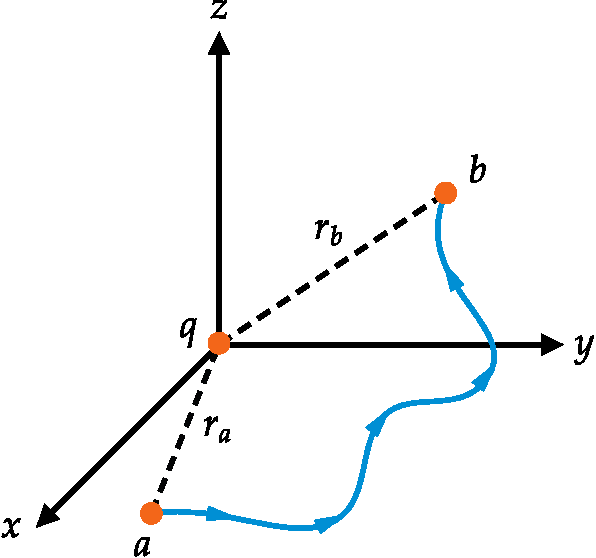
\includegraphics[width=0.35\textwidth]{curl of electric field}
	\end{center}
	\caption{curl of electric field}
\end{wrapfigure}

Consider a point charge situated at the origin, then electric field at a distance $r$ is given by,
\begin{align*}
\vec{E}=\frac{1}{4 \pi \varepsilon_{0}} \frac{q}{r^{2}} \hat{r}
\intertext{Now we will calculate the line integral of this field from  $a$ to $b$ as shown in the figure.}
\int_{{a}}^{{b}} \vec{E}& \cdot \vec{d {l}} \\
\text{In spherical coordinates,} \quad \vec{d {l}}&=d r \hat{{r}}+r d \theta \hat{{\theta}}+r \sin \theta d \phi \hat{{\phi}}\\ 
\text{So}\quad
\vec{E} \cdot \vec{d {l}}&=\frac{1}{4 \pi \epsilon_{0}} \frac{q}{r^{2}} d r\\
\therefore \int_{{a}}^{{b}} \vec{E} \cdot \vec{d {l}}&=\frac{1}{4 \pi \epsilon_{0}} \int_{{a}}^{{b}} \frac{q}{r^{2}} d r\\&=\left.\frac{-1}{4 \pi \epsilon_{0}} \frac{q}{r}\right|_{r_{a}} ^{r_{b}}\\&=\frac{1}{4 \pi \epsilon_{0}}\left(\frac{q}{r_{a}}-\frac{q}{r_{b}}\right)
\end{align*}
Where $r_{a}$ is the distance from the origin to the point ${a}$ and $r_{b}$ is the distance to ${b}$. The integral around a closed path is evidently zero (for then $r_{a}=r_{b}$ ):
\begin{align*}
\oint \vec{E} \cdot \vec{d {l}}&=0\\
\text{On applying Stokes} &\text{ theorem, we get,}
\end{align*}
\begin{center}
	\framebox{
		\parbox[t][0.75cm]{4cm}{
			
			\addvspace{0.2cm} \centering 
			
			$\nabla\times \vec{E}=0$} }
\end{center}
Since, the curl of electric field is zero, an electric field is a conservative field.
\begin{note}
	The curl of Electric field obeys the principle of superposition,
	$\vec{E}=\vec{E}_{1}+\vec{E}_{2}+\ldots$\\Thus,\\
	$\nabla \times \vec{E}=\nabla \times\left(\vec{E}_{1}+\vec{E}_{2}+\ldots\right)=\left(\nabla \times \vec{E}_{1}\right)+\left(\nabla \times \vec{E}_{2}\right)+\ldots=0$
\end{note}
\section{Electric potential}
\begin{definition}
	Electric potential is the amount of workdone need to bring a positive unit charge from infinity to a specific point.\\
We know that $\oint \vec{E} \cdot d \vec{r}=0$, the line integral is independent of path.
	\\So, we can define a function
	\begin{equation}
	V(r)=-\int_{O}^{p} \vec{E} d \vec{r}
	\end{equation} 
	where $O$ is some standard reference point $V$ then depends only on the point $r .$ It is called the
	electric potential.
\end{definition}
Then the potential difference between two points is,\\
$\begin{aligned} V({b})-V({a}) &=-\int_{{O}}^{{b}} \vec{E} \cdot d \vec{r}+\int_{{O}}^{{a}} \vec{E} \cdot d \vec{r} \\ &=-\int_{{O}}^{{b}} \vec{E} \cdot d \vec{r}-\int_{{a}}^{{O}} \vec{E} \cdot d \vec{r}=-\int_{{a}}^{{b}} \vec{E} \cdot d \vec{r} . \end{aligned}$\\
By the fundamental theorem of gradients,
\begin{align*}
V({b})-V({a})&=\int_{a}^{b}(\nabla V) \cdot d \vec{r} \\
\int_{{a}}^{{b}}(\nabla V) \cdot d {r}&=-\int_{{a}}^{{b}} \vec{E} \cdot d \vec{r}\\
\Longrightarrow \vec{E}&=-(\nabla V)
\end{align*}
\begin{center}
	\framebox{
		\parbox[t][0.75cm]{4cm}{
			
			\addvspace{0.2cm} \centering 
			
			$\vec{E}=-(\nabla V)$} }
\end{center}
\begin{itemize}
	\item Electric potential is a scalar quantity.
	\item The potential and potential energy are totally different entities. The name "potential" is very similar to the phrase "potential energy" and this is often confusing because, though there is a connection between the two, they are different things. The relationship is understood by considering the work that needs to be done to bring a test charge q from the reference point to the point $\mathrm{P}$ where it is to be placed, The work done by an external agency then becomes the potential energy of the system. Thus the potential at a point can be interpreted as the potential energy associated with a unit point charge at that point.
	
	\item A surface over which the potential is constant is called
	an equipotential surafce.
	\item Electric potential satisfies the principle of superposition, $$V=V_{1}+V_{2}+\ldots$$
	\item Unit of potential is newton-meters/coulomb or jules/coulomb or volt.
\end{itemize}
In short we can say that, The electric field being a conservative field, its curl is zero. Thus we can  express $\vec{E}$ as a gradient of a scalar field, which we call as the electric potential. By convention to take the electric field as the negative gradient of potential, $\vec{E}=-\vec{\nabla} V$. 
\subsection{Electric potential due to point charge}
\begin{wrapfigure}{r}{0.40\textwidth}
	\begin{center}
		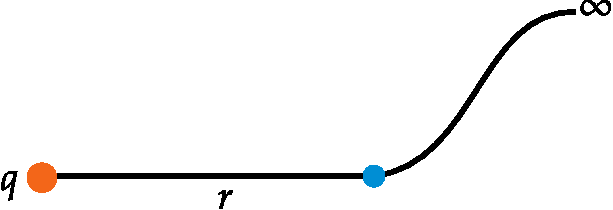
\includegraphics[width=0.30\textwidth]{electric potential1}
	\end{center}
	\caption{Electric potential due to a point charge}
\end{wrapfigure}
The electric potential due to a point charge $q$ at origin at a distance $r$ is
\begin{align*}
V(r)&=-\int_{\infty}^{r} \vec{E} d \vec{r}\\
\text{Here, }E&=\frac{1}{4\pi \epsilon_{0}}\frac{q}{r^{2}}\\
\text{then,}\quad  V(r)&=- \frac{q}{4\pi \epsilon_{0}}\int_{\infty}^{r} 
\frac{ d \vec{r}}{r^{2}}\\
&=\frac{1}{4\pi \epsilon_{0}}\left[ \frac{q}{r} \right]_{\infty}^{r}\\
&=\frac{1}{4\pi \epsilon_{0}} \frac{q}{r} \\
\text{For continuous }&\text{charge distribution,}\\
{V}({r})&=\frac{1}{4 \pi \epsilon_{0}} \int_{{P}} \frac{\lambda\left({r}\right)}{r} \hat{{r}} d l\quad\rightarrow \text{Linear charge distribution.}\\
{V}({r})&=\frac{1}{4 \pi \epsilon_{0}} \int_{{S}} \frac{\sigma\left({r}\right)}{r} \hat{{r}} d a\quad\rightarrow \text{Surface charge distribution.}\\
{V}({r})&=\frac{1}{4 \pi \epsilon_{0}} \int_{{V}} \frac{\rho\left({r}\right)}{r} \hat{r} d \tau\quad \rightarrow \text{Volume charge distribution.}
\end{align*}



\subsection{Electric potential calculation}

\subsubsection{Uniformely charged spherical shell}
Consider a uniformly charged spherical shell having radius $\mathrm{R}$ and charge density$\rho$. Then,
\begin{align*}
\text{Charge density}&:\rho=\frac{Q}{\frac{4}{3} \pi R^{3}}\\
\text{Electric field}&:\text { For } r>R , \quad E_{out}=\frac{Q}{4 \pi \varepsilon_{0} r^{2}}
\\&\text {For}\quad r<R, \quad E_{in}=0
\\&\text {For}\quad r=R, \quad E_{on}=\frac{Q}{4 \pi \varepsilon_{0} R^{2}}\\
\text{Then the potentials are,}\\
	\bullet\text { For } r>R:\\
	V_{out}&=-\int_{\infty}^{r} \vec{E}\cdot d \vec{r}\\
	&=-\int_{\infty}^{r} \frac{Q}{4 \pi \varepsilon_{0} r^{2}}\cdot d {r}\\
	&=\frac{Q}{4 \pi \varepsilon_{0} r}
	\end{align*}
    \begin{align*}
 	\bullet	\text { For } r<R:\\
	V_{in}&=-\int_{\infty}^{R} \vec{E}\cdot d \vec{r}-\int_{R}^{r} \vec{E}\cdot d \vec{r}\\
	&=-\int_{\infty}^{R} \frac{Q}{4 \pi \varepsilon_{0} r^{2}} \cdot d {r}\\
	&=\frac{Q}{4 \pi \varepsilon_{0} R}
	\end{align*}
	 \begin{align*}
		\bullet \text { For } r=R:\\
	V_{on}&=-\int_{\infty}^{R} \vec{E}\cdot d \vec{r}\\
	&=-\int_{\infty}^{R} \frac{Q}{4 \pi \varepsilon_{0} R^{2}}\cdot d {r}\\
	&=\frac{Q}{4 \pi \varepsilon_{0} R}
	\end{align*}

\begin{center}
\framebox{
	\parbox[t][1.5cm]{8cm}{
		
		\addvspace{0.2cm} \centering 
		
		
	$V_{in}=\frac{Q}{4 \pi \varepsilon_{0} R}  ;\quad V_{on}=\frac{Q}{4 \pi \varepsilon_{0} R};\quad  V_{out}=\frac{Q}{4 \pi \varepsilon_{0} r}$} }
\end{center}
\subsubsection{Uniformely charged Solid sphere}
For a uniformely charged solid sphere of radius $R$ the elctric fields are,
\begin{align*}
	\text{Charge density}&:\rho=\frac{Q}{\frac{4}{3} \pi R^{3}}\\
	\text{Electric field}&:\text { For, } r>R=E=\frac{Q}{4 \pi \varepsilon_{0} r^{2}}
	\\&\text {For}\quad r<R, \quad E=\frac{Qr}{4 \pi \varepsilon_{0} R^{3}}
	\end{align*}
 \begin{align*}
	\bullet\text { For ,}\quad r>R:\\
	V_{in}&=-\int_{\infty}^{r} \vec{E}\cdot d \vec{r}\\
	&=-\int_{\infty}^{r} \frac{Q}{4 \pi \varepsilon_{0} r^{2}}\cdot d {r}\\
	&=\frac{Q}{4 \pi \varepsilon_{0} r}\\
	\text{In terms }&\text{of charge density,}\\
	V_{in}&=\frac{\rho R^{3}}{3\epsilon_{0} r}
\end{align*}
 \begin{align*}
	\bullet	\text { For, } \quad r<R:\\
	V_{out}&=-\int_{\infty}^{R} \vec{E}\cdot d \vec{r}-\int_{R}^{r} \vec{E}\cdot d \vec{r}\\
	&=-\int_{\infty}^{R} \frac{Q}{4 \pi \varepsilon_{0} r^{2}}\cdot d {r}-\int_{R}^{r} \frac{Qr}{4 \pi \varepsilon_{0} R^{3}} \cdot d {r}\\
	&=\frac{Q}{4 \pi \varepsilon_{0} R}-\left[\frac{Q }{4 \pi \varepsilon_{0} R^{3}} \frac{r^{2}}{2} \right]_{R}^{r}\\
		&=\frac{Q}{4 \pi \varepsilon_{0} R}-\left[\frac{Q }{4 \pi \varepsilon_{0} R^{3}} \frac{r^{2}}{2} \right]+\left[\frac{Q }{4 \pi \varepsilon_{0} R^{3}} \frac{R^{2}}{2} \right]\\ 
		&=\frac{Q }{4 \pi \varepsilon_{0}}\left[\frac{3}{2R}-\frac{r^{2}}{2R^{3}} \right]\\ 
		&=\frac{Q }{8 \pi \varepsilon_{0}R^{3}}\left[3R^{2}-r^{2} \right]\\
	\text{In terms of}&\text{ charge density,}\\
	V_{out}&=\frac{\rho }{6  \varepsilon_{0}}\left[3R^{2}-r^{2} \right]
\end{align*}
\begin{note}
$	V_{at centre}=\frac{3}{2}\frac{Q}{4 \pi \varepsilon_{0} R}\\
	V_{at centre}=\frac{3}{2}V_{on}$
\end{note}
\subsubsection{Uniformely charged  Circular disc}

Consider a Uniformely charged  Circular disc of charge density $\sigma$.Let us take an circular segment of radius $r$ and $r+d r$. The potential due to this element is\\
\begin{minipage}{0.65\textwidth}
\begin{align*}
d V&=\frac{1}{4 \pi \varepsilon_{0}} \frac{\sigma da}{\sqrt{r^{2}+z^{2}}} \quad \Longrightarrow \quad da=d(\pi r^{2})=2\pi r dr \\
d V&=\frac{1}{4 \pi \varepsilon_{0}} \frac{ \sigma 2 \pi r d r }{\sqrt{r^{2}+z^{2}}} \\
V&=\frac{1}{4 \pi \varepsilon_{0}} 2 \pi \sigma \int_{0}^{R} \frac{2 r d r}{\sqrt{z^{2}+r^{2}}}=\frac{\sigma}{2 \varepsilon_{0}}\left[\sqrt{z^{2}+r^{2}}\right]_{0}^{R} \\
&=\frac{\sigma}{2 \varepsilon_{0}}\left(\sqrt{z^{2}+R^{2}}-|z|\right)\\
\end{align*}
\end{minipage}
\begin{minipage}{0.35\textwidth}
	\begin{figure}[H]
		\centering
	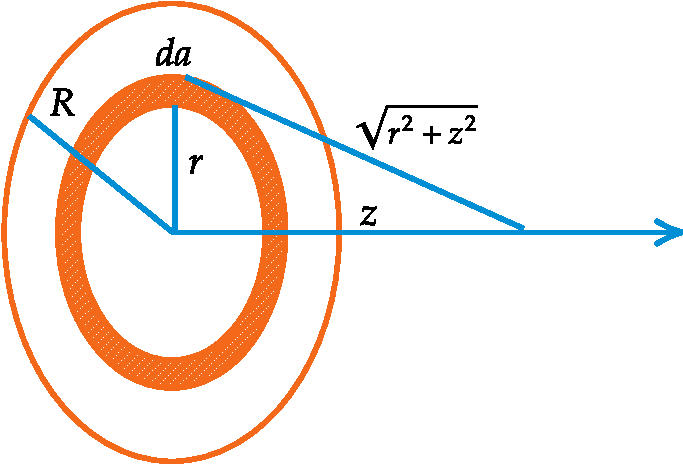
\includegraphics[width=0.85\textwidth]{circular disc}
		\caption{Uniformely charged circular disc}
		\label{charged circular disc}
	\end{figure}
	
\end{minipage}


\begin{exercise}
	Three concentric metallic shells $A, B$ and $C$ of radii $a, b$, and $c(a<b<c)$ have surface charge densities
	$\sigma,-\sigma$ and $\sigma$ respectively.\\
	(\textbf{1}) Find the potentials of three shells $A, B$ and $C$\\
	(\textbf{2}) If the shells $A$ and $C$ are at the same potential, obtain the relation between the radii $a, b$ and $c .$
	\begin{figure}[H]
		\begin{center}
			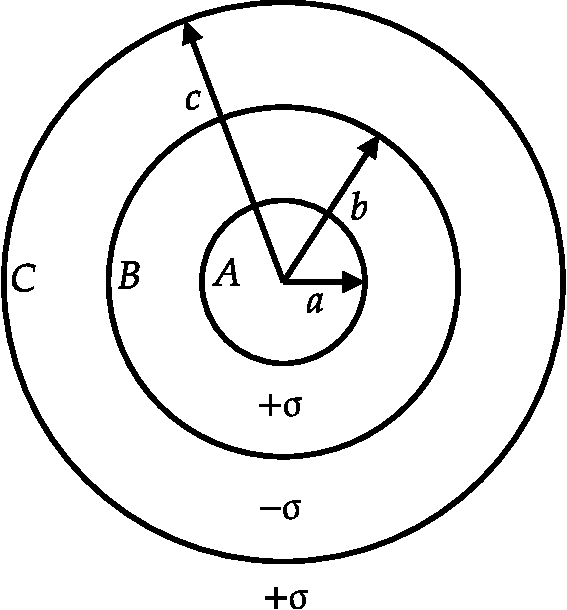
\includegraphics[width=0.25\textwidth]{exercise e-field1}
		\end{center}
	\end{figure}
\end{exercise}
\begin{answer}\textbf{1.}\\
	\begin{align*}
	\text{Potential of } A =&(\text{Potential of } A \text{ due to }+\sigma \text{ on }A)+(\text{Potential of } A \text{ due to }-\sigma \text{ on }B)\\&+(\text{Potential of } A \text{ due to }+\sigma \text{ on }C)\\
	=&\frac{1}{4 \pi \varepsilon_{0}}\left[\frac{4 \pi a^{2} \sigma}{a}-\frac{4 \pi b^{2} \sigma}{b}+\frac{4 \pi c^{2} \sigma}{c}\right]\\
	=&\frac{\sigma}{\varepsilon_{0}}[a-b+c]
	\end{align*}
	\begin{align*}
\text{Potential of } B =&( \text{Potential due to} +\sigma \text{on} A)+( \text{Potential due to} -\sigma \text{on} B)\\&+( \text{Potential due to} +\sigma \text{on} C)\\
=&\frac{1}{4 \pi \varepsilon_{0}}\left[\frac{4 \pi a^{2} \sigma}{b}-\frac{4 \pi b^{2} \sigma}{b}+\frac{4 \pi c^{2} \sigma}{c}\right]\\
=&\frac{\sigma}{\varepsilon_{0}}\left[\frac{a^{2}}{b}-b+c\right]
	\end{align*}
	\begin{align*}	
	\text{Potential of } C =&( \text{Potential due to}  +\sigma \text{ on } A)+( \text{Potential due to} -\sigma \text{ on } B)\\&+( \text{Potential due to} +\sigma \text{ on } C)\\
	=&\frac{1}{4 \pi \varepsilon_{0}}\left[\frac{4 \pi a^{2} \sigma}{c}-\frac{4 \pi b^{2} \sigma}{c}+\frac{4 \pi c^{2} \sigma}{c}\right]\\
	=&\frac{\sigma}{\varepsilon_{0}}\left[\frac{a^{2}}{c}-\frac{b^{2}}{c}+c\right]
	\end{align*}
	\textbf{2.}\\
	\begin{align*}
		\text { Given that, } V_{A}&=V_{C}\\
		\frac{\sigma}{\varepsilon_{0}}[a-b+c]&=\frac{\sigma}{\varepsilon_{0}}\left[\frac{a^{2}}{c}-\frac{b^{2}}{c}+c\right] \text { or } a-b-c=\frac{a^{2}}{c}-\frac{b^{2}}{c}+c\\
		\text { Solving we get } c&=(a+b) \text { . }
	\end{align*}

	
\end{answer}
\subsection{Laplace and Poisson's eqautions}
The electric field is related to the charge density by the  differential form of Gauss' law as,
\begin{equation}
\left(\vec{\nabla} \cdot \vec{E}=\frac{\rho}{\varepsilon_{0}}\right)\label{gauss law}
\end{equation}
And from the idea of conservative field we know that,\begin{equation}
\vec{E}=-\vec{\nabla} \phi\label{electric field}
\end{equation} 
Then putting, \ eq.\ref{electric field} in eq.\ref{gauss law} we get,
\begin{equation}
-\vec{\nabla} \cdot \vec{\nabla} \phi=\frac{\rho}{\varepsilon_{0}}\quad \Longrightarrow \quad \nabla^{2} \phi=-\frac{\rho}{\varepsilon_{0}}\label{poissons} 
\end{equation}
The eq \ref{poissons} is known as the Poisson's equation. 

\begin{center}
\framebox{
	\parbox[t][0.75cm]{4cm}{
		
		\addvspace{0.2cm} \centering 
		$\nabla^{2} \phi=-\frac{\rho}{\varepsilon_{0}}$} }
\end{center}
Laplace's equation follows from Poisson's equation in the region where there is no charge density $\rho=0 .$ The solutions of Laplace's equation are called harmonic functions. If we put $\rho=0$ in eq.\ref{poissons},  then we get,
\begin{center}
	\framebox{
		\parbox[t][0.75cm]{4cm}{
			
			\addvspace{0.2cm} \centering 
			
			$
			\nabla^{2} \phi=0
			$} }
\end{center}
\begin{note}
This mathematical operation,$ \nabla^{2}$, the divergence of the gradient of a function, is called the Laplacian.
\end{note}
\section{Laplace equation in different co-ordinate systems}
\subsection{Laplace's Equation in One Dimension}
Suppose $V$ depends on only one variable, $x$. Then Laplace's equation becomes
\begin{align*}
\frac{d^{2} V}{d x^{2}}&=0\\
\text{The general }&\text{solution is}\\
V(x)&=m x+b,
\end{align*}
the equation for a straight line. It contains two undetermined constants $(m$ and $b)$, as is appropriate for a second-order (ordinary) differential equation. They are fixed, in any particular case, by the boundary conditions of that problem.\\
I want to call your attention to two features of this result; they may seem silly and obvious in one dimension, where I can write down the general solution explicitly, but the analogs in two and three dimensions are powerful and by no means obvious:
1. $V(x)$ is the average of $V(x+a)$ and $V(x-a)$, for any $a$ :
$$
V(x)=\frac{1}{2}[V(x+a)+V(x-a)] .
$$
Laplace's equation is a kind of averaging instruction; it tells you to assign to the point $x$ the average of the values to the left and to the right of $x$. Solutions to Laplace's equation are, in this sense, as boring as they could possibly be, and yet fit the end points properly.
2. Laplace's equation tolerates no local maxima or minima; extreme values of $V$ must occur at the end points. Actually, this is a consequence of (1), for if there were a local maximum, $V$ at that point would be greater than on either side, and therefore could not be the average.
\subsection{Laplace's Equation in Two Dimensions}
If $V$ depends on two variables, Laplace's equation becomes
$$
\frac{\partial^{2} V}{\partial x^{2}}+\frac{\partial^{2} V}{\partial y^{2}}=0
$$
This is no longer an ordinary differential equation (that is, one involving ordinary derivatives only); it is a partial differential equation. As a consequence, some of the simple rules you may be familiar with do not apply. For instance, the general solution to this equation doesn't contain just two arbitrary constants-or, for that matter, any finite number-despite the fact that it's a second-order equation. Indeed, one cannot write down a "general solution" . Nevertheless, it is possible to deduce certain properties common to all solutions.\\
1. The value of $V$ at a point $(x, y)$ is the average of those around the point. More precisely, if you draw a circle of any radius $R$ about the point $(x, y)$, the average value of $V$ on the circle is equal to the value at the center:
$$
V(x, y)=\frac{1}{2 \pi R} \oint_{\text {circle }} V d l .
$$
2. $V$ has no local maxima or minima; all extrema occur at the boundaries. (As before, this follows from (1).) Again, Laplace's equation picks the most featureless function possible, consistent with the boundary conditions: no hills, no valleys, just the smoothest surface available.
\section{Laplace's Equation in Three Dimensions}
In three dimensions I can neither provide you with an explicit solution (as in one dimension) nor offer a suggestive physical example to guide your intuition (as I did in two dimensions). Nevertheless, the same two properties remain true, and this time I will sketch a proof.\\\\
1. The value of $V$ at point $\mathbf{r}$ is the average value of $V$ over a spherical surface of radius $R$ centered at $\mathbf{r}$ :
$$
V(\mathbf{r})=\frac{1}{4 \pi R^{2}} \oint_{\text {sphere }} V d a .
$$
2. As a consequence, $V$ can have no local maxima or minima; the extreme values of $V$ must occur at the boundaries. (For if $V$ had a local maximum at $\mathbf{r}$, then by the very nature of maximum I could draw a sphere around $\mathbf{r}$ over which all values of $V$-and a fortiori the average-would be less than at $\mathbf{r}$.)\\\\
Proof: Let's begin by calculating the average potential over a spherical surface of radius $R$ due to a single point charge $q$ located outside the sphere. We may as well center the sphere at the origin and choose coordinates so that $q$ lies on the $z$-axis . The potential at a point on the surface is
\begin{align*}
V&=\frac{1}{4 \pi \epsilon_{0}} \frac{q}{r}\\
\text{ where }\quad
r^{2}&=z^{2}+R^{2}-2 z R \cos \theta,\\
\text{ so }\quad
V_{\text {ave }} &=\frac{1}{4 \pi R^{2}} \frac{q}{4 \pi \epsilon_{0}} \int\left[z^{2}+R^{2}-2 z R \cos \theta\right]^{-1 / 2} R^{2} \sin \theta d \theta d \phi \\
&=\left.\frac{q}{4 \pi \epsilon_{0}} \frac{1}{2 z R} \sqrt{z^{2}+R^{2}-2 z R \cos \theta}\right|_{0} ^{\pi} \\
&=\frac{q}{4 \pi \epsilon_{0}} \frac{1}{2 z R}[(z+R)-(z-R)]=\frac{1}{4 \pi \epsilon_{0}} \frac{q}{z}
\end{align*}
But this is precisely the potential due to $q$ at the center of the sphere! By the superposition principle, the same goes for any collection of charges outside the sphere: their average potential over the sphere is equal to the net potential they produce at the center. 
\begin{figure}[H]
	\centering
	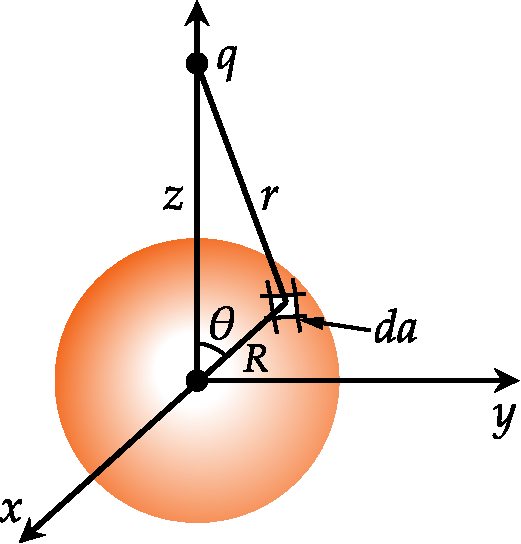
\includegraphics[height=4cm,width=4cm]{electric potential 01}
	\caption{}
	\label{}
\end{figure}
\section{Laplace equation in Spherical polar coordinates}
\begin{align}
\text{In  the spherical polar coordinate system, }&\text{The Laplace equation is,}\\
\frac{1}{r^{2}} \frac{\partial}{\partial r}\left(r^{2} \frac{\partial V}{\partial r}\right)+\frac{1}{r^{2} \sin \theta} \frac{\partial}{\partial \theta}\left(\sin \theta \frac{\partial V}{\partial \theta}\right)&+\frac{1}{r^{2} \sin ^{2} \theta} \frac{\partial^{2} V}{\partial \phi^{2}}=0 \label{Laplace in spc 1}
\intertext{Let us assume the system has an azimuthal symmetry such that \ $V$\ is independent of  $\phi$.Then the solution of the above equation can be written as,}
V(r, \theta)&=R(r) \Theta(\theta)\label{Laplace in spc 2}\\
\text{Dividing equation \ref{Laplace in spc 1} by \  $V$\ ,\ i.e \ref{Laplace in spc 2} , \ we get,}\\
\frac{1}{R} \frac{d}{d r}\left(r^{2} \frac{d R}{d r}\right)+\frac{1}{\Theta \sin \theta} \frac{d}{d \theta}\left(\sin \theta \frac{d \Theta}{d \theta}\right)&=0\\
\text{The above equation can be written as, }\\
\frac{1}{R} \frac{d}{d r}\left(r^{2} \frac{d R}{d r}\right)&=l(l+1)\\ \text{And,}\quad \frac{1}{\Theta \sin \theta} \frac{d}{d \theta}\left(\sin \theta \frac{d \Theta}{d \theta}\right)&=-l(l+1)
\intertext{Here $l(l+1)$ is just a  way of writing the separation constant. By the method of separation of variables, the equation can be  converted into ordinary differential equations. The radial equation is,}
\frac{d}{d r}\left(r^{2} \frac{d R}{d r}\right)&=l(l+1) R\\
\text{It has the general solution,}\\
R(r)&=A r^{l}+\frac{B}{r^{l+1}}
\intertext{	Where $A$ and $B$ are  two arbitrary constants  in the solution of a second-order differential equation. Then the  angular equation,}
\frac{d}{d \theta}\left(\sin \theta \frac{d \Theta}{d \theta}\right)&=-l(l+1) \sin \theta \Theta\\
\text{The solutions are Legendre polynomials in the }&\text{variable $\cos \theta$ :}\\
\Theta(\theta)&=P_{l}(\cos \theta)\\
\text{$P_{l}(x)$ is most conveniently defined by the Rodrigues }&\text{ formula:}\\
P_{l}(x)&=\frac{1}{2^{l} l !}\left(\frac{d}{d x}\right)^{l}\left(x^{2}-1\right)^{l}\\
\Theta(\theta)&=\ln \left(\tan \frac{\theta}{2}\right)\\
\text{In the case of azimuthal symmetry, the most general}&\text{ separable solution to Laplace's equation is,}\\
V(r, \theta)&=\left(A r^{l}+\frac{B}{r^{l+1}}\right) P_{l}(\cos \theta)
\intertext{As before, separation of variables yields an infinite set of solutions,
	one for each $l$. The general solution is the linear combination of separable solutions,}
V(r, \theta)&=\sum_{l=0}^{\infty}\left(A_{l} r^{l}+\frac{B_{l}}{r^{l+1}}\right) P_{l}(\cos \theta)
\end{align}

\begin{note}
	Legendre polynomials values.
	\begin{align*}
	P_{0}(x) & =1 \\
	P_{1}^{\prime}(x) & =x \\
	P_{2}(x) & =\left(3 x^{2}-1\right) / 2 \\
	P_{3}(x) & =\left(5 x^{3}-3 x\right) / 2 \\
	P_{4}(x) & =\left(35 x^{4}-30 x^{2}+3\right) / 8 \\
	P_{5}(x) & =\left(63 x^{5}-70 x^{3}+15 x\right) / 8
	\end{align*}
\end{note}
\begin{note}\textbf{Spherical Polar Coordinate System.}
	\begin{align*}
	\text{If $V$ is only a function}&\text{ of $r$ then,}\\
	\frac{\partial V}{\partial \theta}=0 \quad	\text{And} \quad
	\frac{\partial V}{\partial \phi}&=0\\
	\text{Therefore, Laplace's }&\text{equation can be rewritten as}\\
	\frac{1}{r^{2}} \frac{\partial}{\partial r}\left(r^{2} \frac{\partial V}{\partial r}\right)&=0\\
	r^{2} \frac{\partial V}{\partial r}&=A=\text { constant }\\
	\frac{\partial V}{\partial r}&=\frac{A}{r^{2}}\\
	\text{The general solution}&\text{ of this first-order differential equation is}\\
	V(r)&=-\frac{A}{r}+B
	\intertext{Where $B$ is a constant. If $V=0$ at infinity then $B$ must be equal to zero, and consequently}
	V(r)&=-\frac{A}{r}
	\end{align*}
	\begin{center}
		\framebox{
			\parbox[t][0.75cm]{4cm}{
				
				\addvspace{0.2cm} \centering 
				
				$V(r)=-\frac{A}{r}+B $} }
	\end{center}
\end{note}
\begin{note}
	\textbf{Laplace's equation in cylindrical coordinates is}
	\begin{align*}
	\frac{1}{r} \frac{\partial}{\partial r}\left(r \frac{\partial V}{\partial r}\right)+\frac{1}{r^{2}} \frac{\partial^{2} V}{\partial \phi^{2}}&+\frac{\partial^{2} V}{\partial z^{2}}=0\\
	\text{If $V$ is only a function  }&\text{of $r$ then,}\\
	\frac{\partial V}{\partial \phi}&=0 \\
	\frac{\partial V}{\partial z}&=0\\
	\text{Therefore, Laplace's equation}&\text{ can be rewritten as,}\\
	\frac{1}{r} \frac{\partial}{\partial r}\left(r \frac{\partial V}{\partial r}\right)&=0\\
	\text{This differential equation }&\text{can be rewritten as,}\\
	\frac{\partial V}{\partial r}&=\frac{A}{r}\\
	\text{The general solution of this first-order}&\text{ differential equation is,}\\
	V(r)&=A \ln (r)+B\\
	\text{Where $b$ is a constant. The constants $A$ and $B$ }&\text{are determined by the boundary conditions. }
	\end{align*}
	\begin{center}
		\framebox{
			\parbox[t][0.75cm]{4cm}{
				
				\addvspace{0.2cm} \centering 
				
				$V(r)=A \ln (r)+B $} }
	\end{center}	
\end{note}
\begin{exercise}
	Potential in a region of space is given by, $\phi=\phi_{0} e^{-a x^{2}}$ where $\phi_{0}$ and $a$ is constant. Then
	find the charge density in this region.
\end{exercise}
\begin{answer}
	\begin{align*}
	\nabla^{2} \phi&=-\frac{\rho}{\varepsilon_{0}} \\ \rho&=-\varepsilon_{0}\left(\nabla^{2} \phi\right)\\
	&=2 a \varepsilon_{0} \phi\left(1-2 a x^{2}\right)
	\end{align*}
\end{answer}

\begin{exercise}
	Consider two concentric spherical conducting shells centered at the origin. The outer
	radius of the inner shell is $r_{a}$ and the inner radius of the outer shell is $r_{b}$. The charge ensity
	$\rho=0$ in the region $r_{a}<r<r_{b} .$ If $V=0$ at $r=r_{a}$ and $V=V_{0}$ at $r=r_{b}$, then find $V$ in the
	region $r_{a}<r<r_{b}$.
\end{exercise}
\begin{answer}
	\begin{align*}
	\text {Here voltage is varying only with }& r \text { , then the  Laplace's equation is, }\\
	\nabla^{2} V&=\frac{1}{r^{2}} \frac{d}{d r}\left(r^{2} \frac{d V}{d r}\right)=0\\
	\text{Integrate twice to get  }&\text{the solution}V(r)=- \frac{A}{r}+B\\
	\text{The boundary conditions}&\text{ are}\\
	(1) V&=0 \text{ at } r=r_{a}\\
	(2) V&=V_{0} \text{ at  }r=r_{b}\\
	\text { Substituting these boundary }&\text{ conditions, we get}\\
	\text { At } r=r_{a}, 0&=- \frac{A}{r_{a}}+B \Rightarrow B= \frac{A}{r_{a}}\\
	\text { At } r&=r_{b}, V_{0}=- \frac{A}{r_{b}}+ \frac{A}{r_{a}}=A\left[ \frac{1}{r_{a}}- \frac{1}{r_{b}}\right]\\
	V_{0}&=A \frac{r_{b}-r_{a}}{r_{a} r_{b}}\\
	A&= V_{0}\frac{r_{a} r_{b}}{r_{b}-r_{a}}\\
	\text{Then, the constant B,}\\
	B&=\frac{A}{r_{a}}=V_{0}\frac{ r_{b}}{r_{b}-r_{a}}\\
	\text{Then,}\ V&=-  V_{0}\frac{r_{a} r_{b}}{r_{b}-r_{a}}\frac{1}{r}+V_{0}\frac{ r_{b}}{r_{b}-r_{a}}\\
	&=V_{0}\frac{ r_{b}}{r_{b}-r_{a}}\left[- \frac{r_{a}}{r}+1\right]\\
	V&=V_{0}\frac{ r_{b}}{r_{b}-r_{a}}\left[1- \frac{r_{a}}{r}\right] 
	\end{align*}
\end{answer}
\subsection{Summary of Electrostatics}
In an Electrostatics  there are  three fundamental quantities : $\rho$, $\vec{E}$, and $V$. And we have six formulas interrelating them. These equations are  summarized below.
\begin{figure}[H]
	\begin{center}
		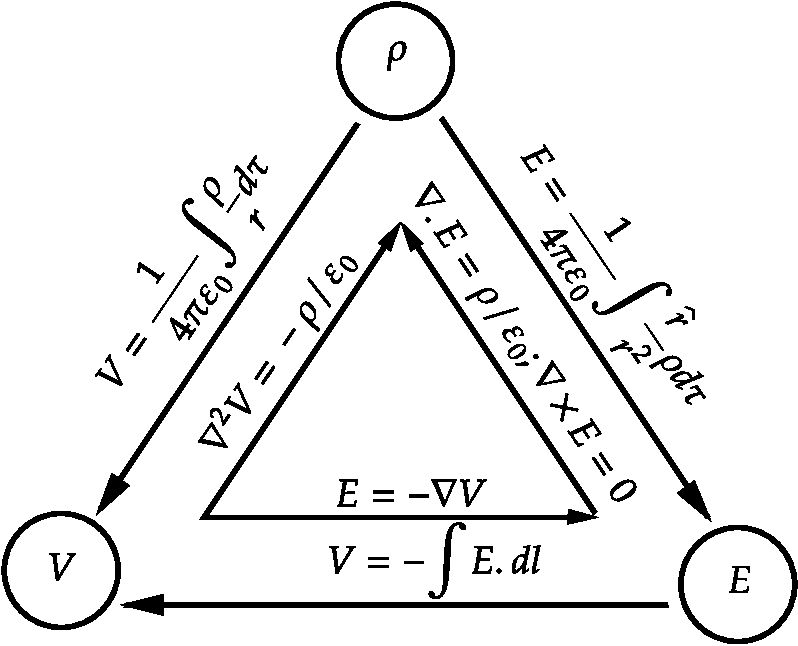
\includegraphics[width=0.45\textwidth]{summary}
	\end{center}
\end{figure}
\subsection{Electrostatic boundary conditions}
\begin{wrapfigure}{r}{0.25\textwidth}
	\begin{center}
		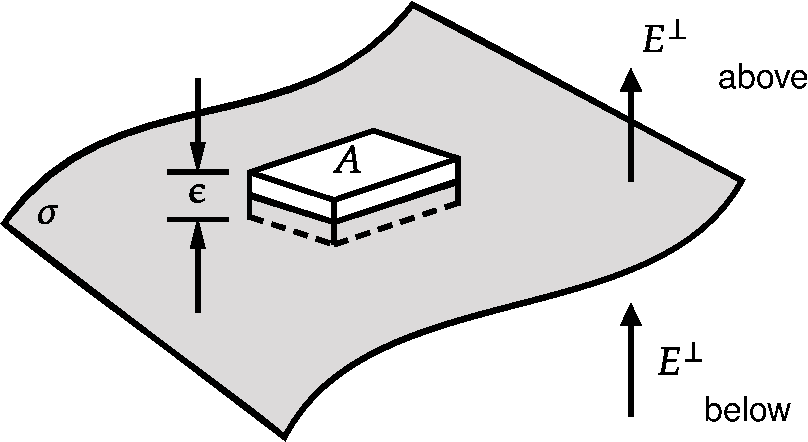
\includegraphics[width=0.30\textwidth]{e boundary3}
	\end{center}
	\caption{Electrostatic boundary}
	\label{Electrostatic boundary1}
\end{wrapfigure}
\textbf{Electric field:}\\\\
The electric field always undergoes a discontinuity when you cross a surface charge $\sigma$. We need to find the amount by which E changes at such a boundary.\\Consider a thin Gaussian pillbox, extending equally above and below the sheet as shown in fig.\ref{Electrostatic boundary1} \\
According to Gauss law,

\begin{align}
\oint_{S} \vec{E} \cdot d \vec{a}=\frac{1}{\epsilon_{0}} Q_{\mathrm{enc}}
&=\frac{1}{\epsilon_{0}} \sigma A \notag\\
\text{\ Then,}\quad  E_{\text {above }}^{\perp} A-E_{\text {below }}^{\perp} A&=\frac{\sigma A}{\varepsilon_{0}}\notag \\
\Rightarrow E_{\text {above }}^{\perp}-E_{\text {below }}^{\perp}&=\frac{\sigma}{\varepsilon_{0}}
\end{align}

\begin{wrapfigure}{r}{0.25\textwidth}
	\begin{center}
		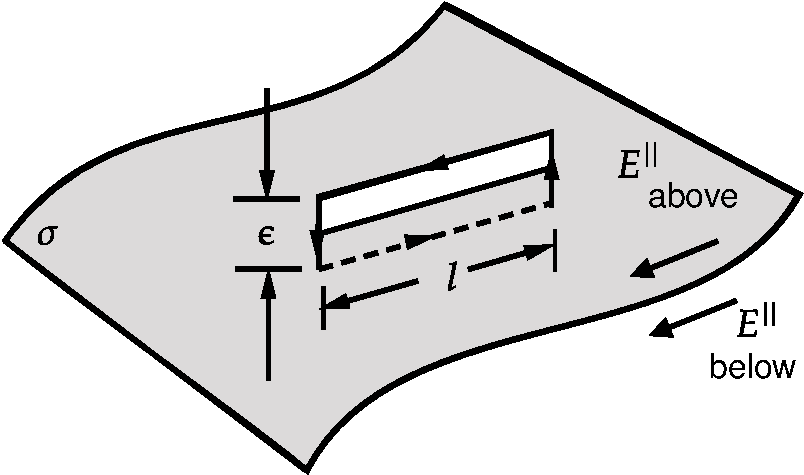
\includegraphics[width=0.30\textwidth]{e boundary1}
	\end{center}
	\caption{Electrostatics}
	\label{Electrostatics boundary 2}
\end{wrapfigure}
\begin{align*}
\text{The tangential component of $E$,}&\text{ by contrast, is always continuous.}\\
\oint \vec{E} \cdot d \vec{l}&=0\\
\intertext{to the thin rectangular loop of Fig.\ref{Electrostatic boundary1}, the ends give nothing $($ as $\epsilon \rightarrow 0)$, and the sides give $\left(E_{\text {above }}^{\|} l-E_{\text {below }}^{\|} l\right)$, so}
{E}_{\text {above }}^{\|}&={E}_{\text {below }}^{\|}\\
\text{Then boundary conditions fo}&\text{ $E$ can be combined into a single formula:}\\
{E}_{\text {above }}-{E}_{\text {below }}&=\frac{\sigma}{\epsilon_{0}} \hat{{n}}\\
\text{where $\hat{n}$ is unit vector }&\text{perpendicular to the surface, pointing upward.}
\end{align*}
\textbf{Conclusions:} 
\begin{itemize}
	\item The normal component of $\vec{E}$ is discontinuous by an amount $\frac{\sigma}{\varepsilon_{0}}$ at any boundary. If there is no surface charge, $E^{\perp}$ is continuous.
	\item The tangential component of $E$,  is always continuous.
\end{itemize}

\opencutright
\renewcommand\windowpagestuff{
	\centering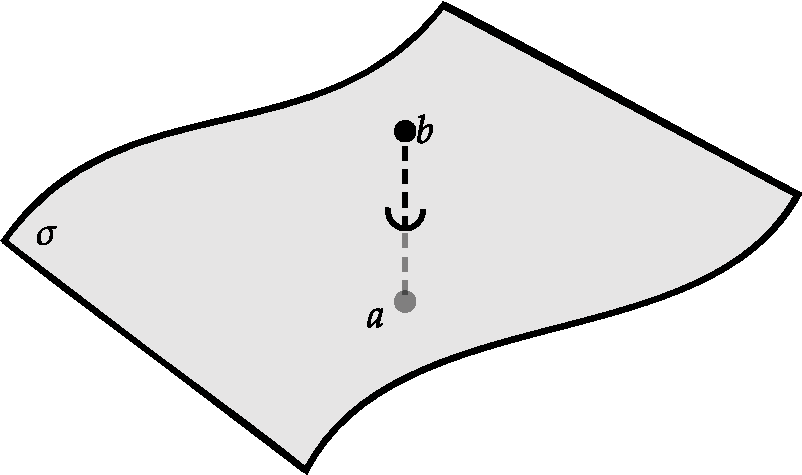
\includegraphics[width=5cm]{e boundary2}}
\begin{cutout}{0}{\dimexpr\linewidth-3.5cm\relax}{0pt}{5}
	\textbf{Potential:}
	
	\begin{align}
	\text{The potential is continuous }&\text{across any boundary, }\notag\\
	\text{Since }\ V_{\text {above }}-V_{\text {below }}&=-\int_{a}^{b} \vec{E} \cdot d \vec{l}\notag\\
	\text{As the path shrinks to zero}\notag\\
	V_{\text {above }}&=V_{\text {below }} \notag\\
	\vec{\nabla} V_{\text {above }}-\vec{\nabla} V_{\text {below }}&=-\frac{\sigma}{\varepsilon_{0}} \hat{n}\hspace{1cm} \because\vec{E}=-\vec{\nabla} V \\
	\nabla V_{\text {above }}-\nabla V_{\text {below }}&=-\frac{1}{\epsilon_{0}} \sigma \hat{n} \notag \\
	\frac{\partial V_{\text {above }}}{\partial n}-\frac{\partial V_{\text {below }}}{\partial n}&=-\frac{1}{\epsilon_{0}} \sigma \notag\\
	\frac{\partial V}{\partial n}&=\nabla V \cdot \hat{{n}}
	\end{align}
	$\frac{\partial V}{\partial n}=\vec{\nabla} V \cdot \hat{n}$ denotes the normal derivative of $V$ (that is the rate of change in the direction perpendicular to the surface.)
\end{cutout}

\begin{center}
	\framebox{
		\parbox[t][4cm]{6cm}{
			
			\addvspace{0.2cm} \centering 
			\begin{align*}
			E_{\text {above }}^{\perp}-E_{\text {below }}^{\perp}&=\frac{\sigma}{\varepsilon_{0}}\\
			{E}_{\text {above }}^{\|}-{E}_{\text {below }}^{\|}&=0\\
			{V}_{\text {above }}-{V}_{\text {below }}&=0\\
			\nabla V_{\text {above }}-\nabla V_{\text {below }}&=-\frac{1}{\epsilon_{0}} \sigma \hat{n}
			\end{align*}
			
	} }
\end{center}








\newpage

\begin{table}[H]
	
	\centering
	\arrayrulecolor{ocre}
	\begin{tabular}{|p{3.5cm}|p{3.8cm}|p{4.6cm}|p{4.2cm}|}
		\hline
		\multicolumn{4}{|c|}{\textbf{Table of Electric field and Potential}}\\\hline\hline
		Uniform charge distribution&Shape and Position of point&Electric field&Electric Potential\\\hline
		\multirow{2}{*}{Line charge}& At a distance $x$ from midpoint of line charge
		$x>>L$\newline 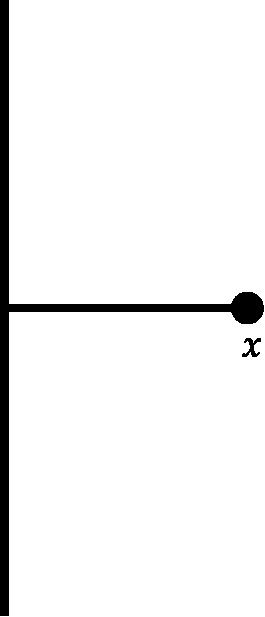
\includegraphics[width=0.05\textwidth]{line charge1}
		&$\frac{1}{4 \pi \varepsilon_{0}} \frac{Q}{x^{2}}$\newline\newline  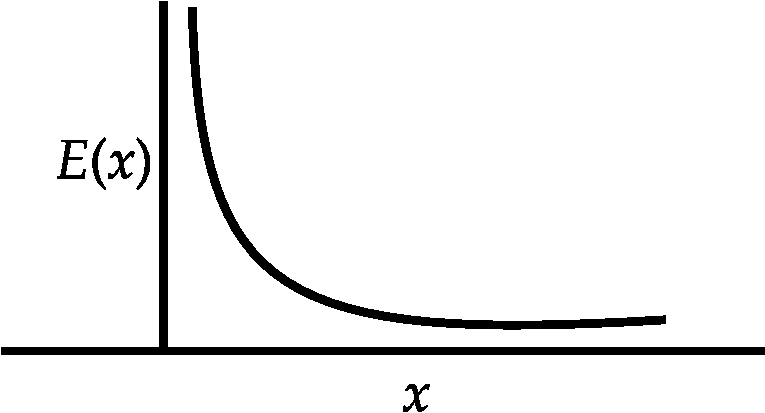
\includegraphics[width=0.20\textwidth]{line charge1electric field}&$\frac{1}{4 \pi \varepsilon_{0}} \frac{Q}{x}$\newline\newline  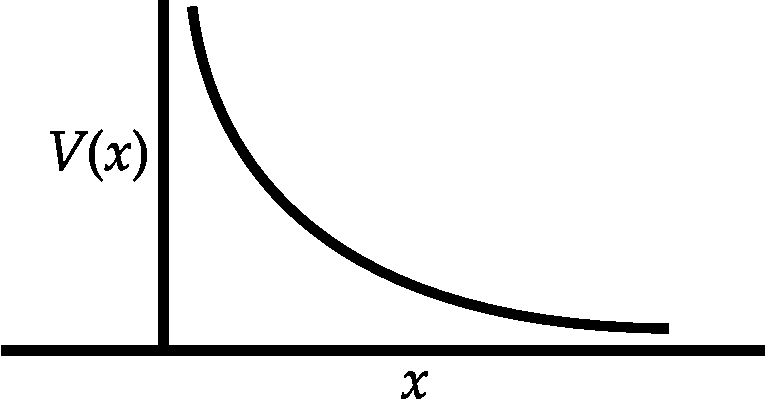
\includegraphics[width=0.20\textwidth]{line charge1potential}\\\cline{2-4}
		
		&At a distance $x$ from the one end of\newline \newline 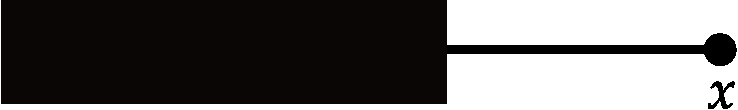
\includegraphics[width=0.20\textwidth]{line charge2}   &$\frac{1}{4 \pi \varepsilon_{0}} \frac{Q}{x(L+x)}$\newline \newline 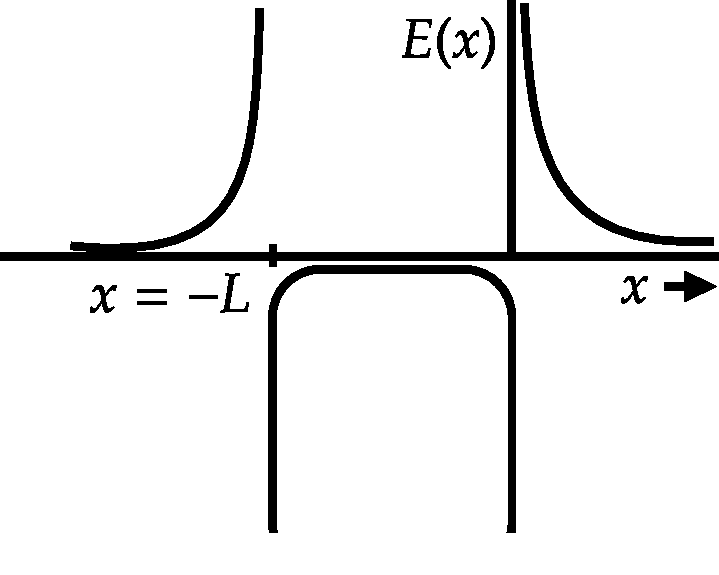
\includegraphics[width=0.20\textwidth]{line charge2electric field}   &$\frac{1}{4 \pi \varepsilon_{0}} \frac{Q}{L} \ln \left(1+\frac{L}{x}\right)$ \newline\newline 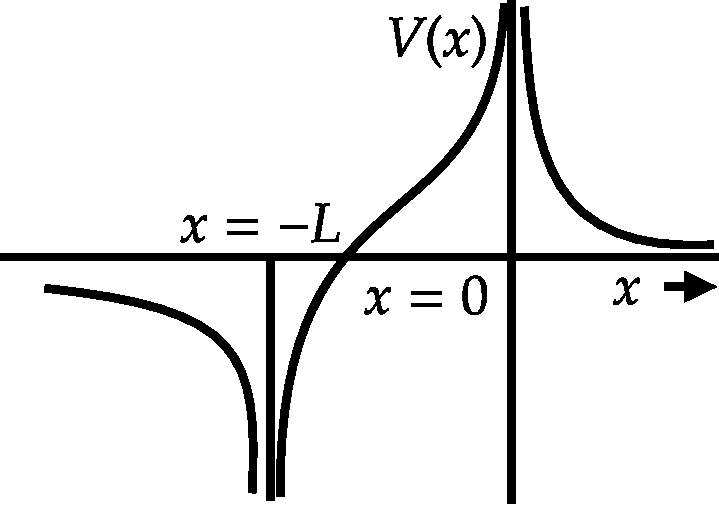
\includegraphics[width=0.20\textwidth]{line charge2potential} \\\hline
		
		Charged ring&On the axis at a distance $\mathrm{x}$ from
		centre \newline\newline 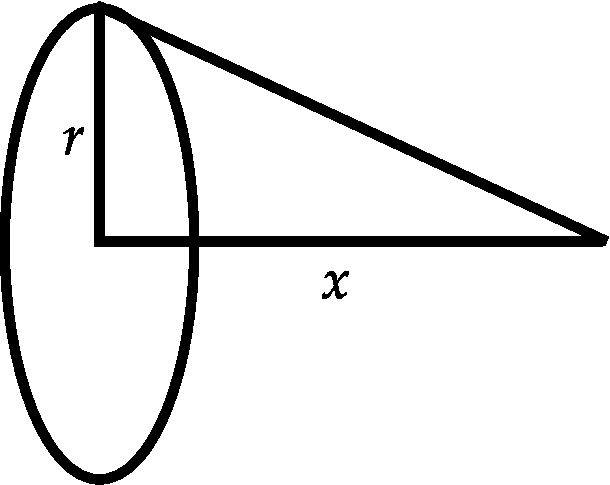
\includegraphics[width=0.15\textwidth]{chargedring}  &$\frac{1}{4 \pi \varepsilon_{0}} \frac{Q x}{\left(r^{2}+x^{2}\right)^{3 / 2}} $ \newline\newline 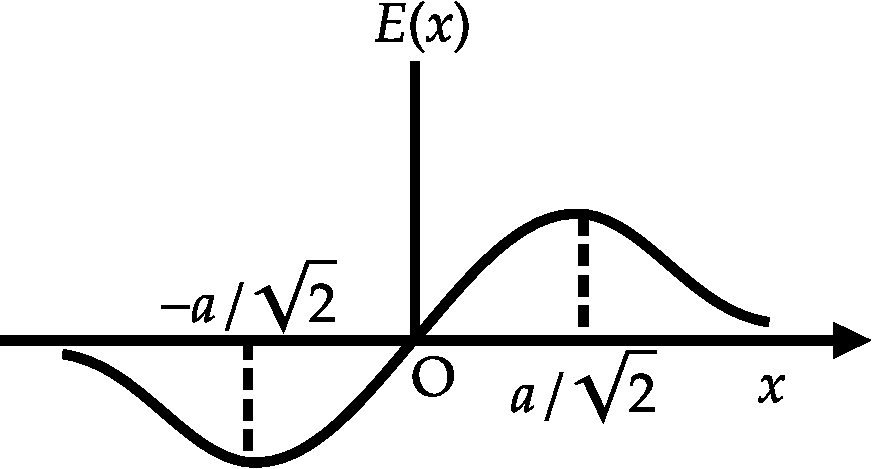
\includegraphics[width=0.20\textwidth]{chargedringelectricfield} &$\frac{1}{4 \pi \varepsilon_{0}} \frac{Q}{\sqrt{r^{2}+x^{2}}}$ \newline\newline 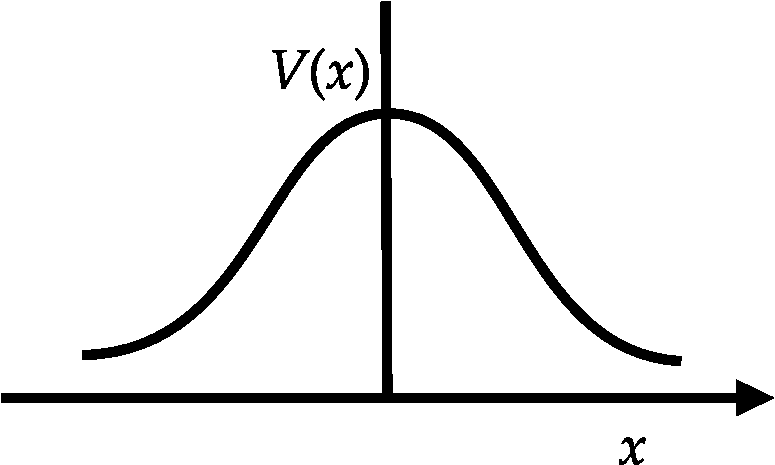
\includegraphics[width=0.20\textwidth]{chargedringpotential}\\\hline
		
		Charged disc& On the axis at  a distance $x$ from centre\newline\newline 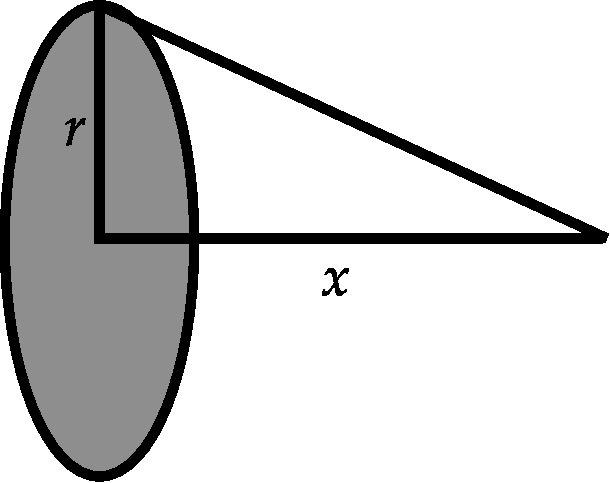
\includegraphics[width=0.17\textwidth]{charged disc} &$
		\begin{array}{l}
		\frac{\sigma}{2 \varepsilon_{0}}\left[1-\frac{x}{\sqrt{r^{2}+x^{2}}}\right] x \text { for } x>0 \\
		-\frac{\sigma}{2 \varepsilon_{0}}\left[1+\frac{x}{\sqrt{r^{2}+x^{2}}}\right] x \text { for } x<0
		\end{array}
		$ \newline\newline 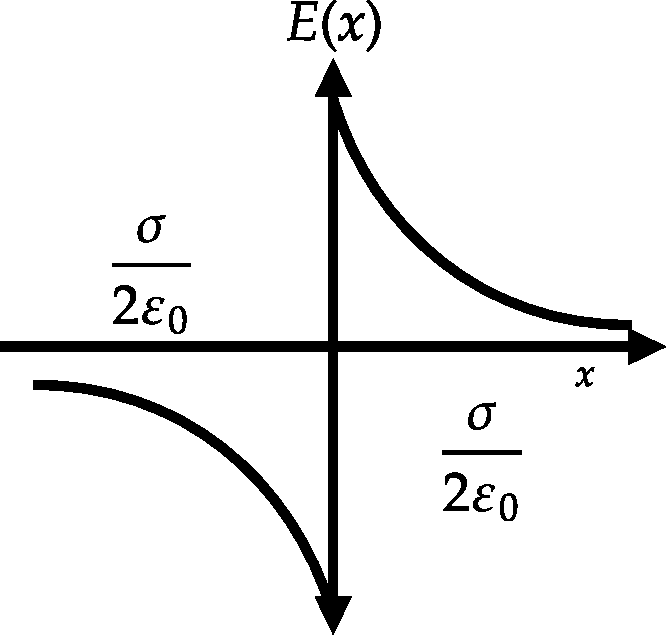
\includegraphics[width=0.20\textwidth]{charged discelectricfied}  &$\frac{\sigma}{2 \varepsilon_{0}}\left[\sqrt{r^{2}+x^{2}}-x\right]$ \newline\newline 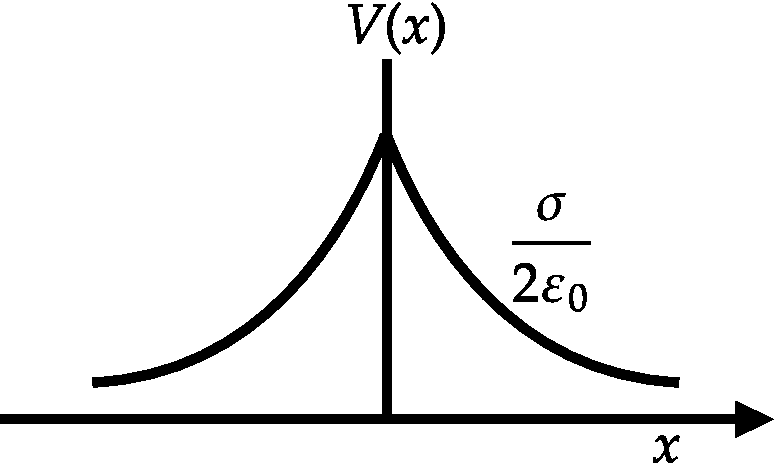
\includegraphics[width=0.20\textwidth]{charged discpotential} \\\hline
		
		
		\multirow{2}{*}{	Charged solid sphere}& Outside the sphere
		\newline 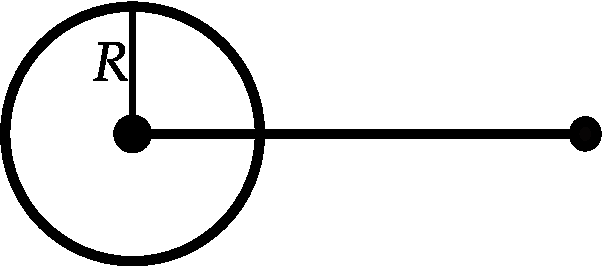
\includegraphics[width=0.15\textwidth]{hollowsphereout}
		&$\frac{1}{4 \pi \varepsilon_{0}} \frac{Q}{r^{2}}$ for $r>R$&$\frac{1}{4 \pi \varepsilon_{0}} \frac{Q}{r} $ for $r>R$\\
		&Inside the sphere\newline \newline 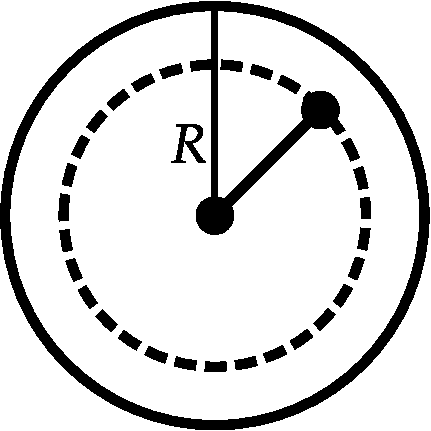
\includegraphics[width=0.09\textwidth]{hollowspherein}   & $\frac{1}{4 \pi \varepsilon_{0}} \frac{Qr}{R^{3}}$for $r<R$\newline \newline 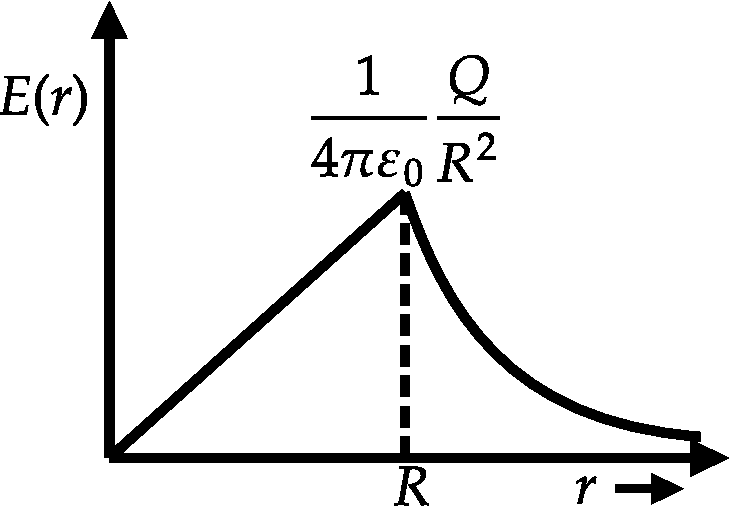
\includegraphics[width=0.18\textwidth]{hollowsphereinelectricfield}   &$\frac{Q}{4 \pi \varepsilon_{0} R}\left[\frac{3}{2}-\frac{r^{2}}{2 R^{2}}\right]$for $r<R$ \newline\newline 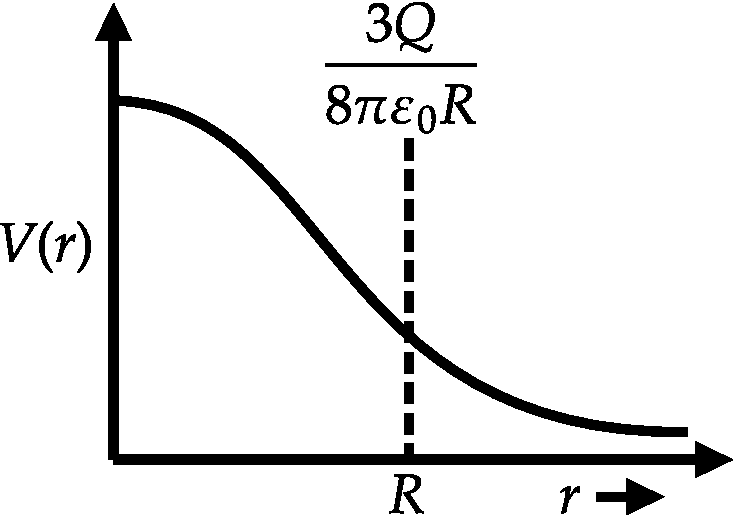
\includegraphics[width=0.18\textwidth]{hollowsphereinpotential} \\\hline
		
		\multirow{2}{*}{Charged solid cylinder}& Inside the cylinder
		\newline 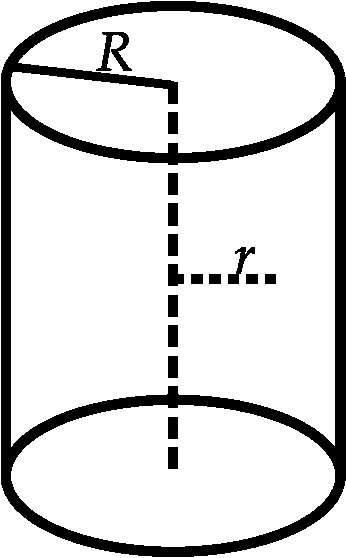
\includegraphics[width=0.07\textwidth]{solidcylinderin}\newline Outside the cylinder\newline \newline 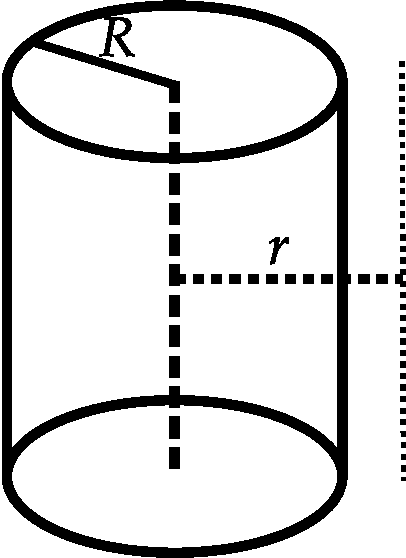
\includegraphics[width=0.08\textwidth]{solidcylinderout} 
		&$\frac{\rho r}{2 \varepsilon_{0}}$ for $r<R$  \newline \newline $\frac{\rho R^{2}}{2 \varepsilon_{0}r}$ for $r>R$\newline \newline
		
		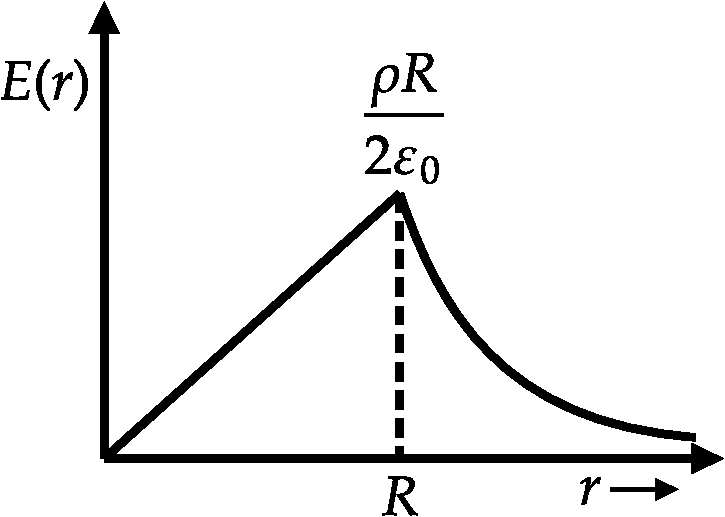
\includegraphics[width=0.20\textwidth]{solidcylinderelectricfield} &$\frac{R^{2} \rho}{2 \varepsilon_{0}} \operatorname{ln}\left(\frac{r_{0}}{R}\right)+\frac{\rho}{4 \varepsilon_{0}}\left(R^{2}-r^{2}\right)$ for $r<R$ \newline \newline $\frac{a^{2} \rho}{2 \varepsilon_{0}}\left(\ln\left(\frac{r_{0}}{r}\right)\right.$for $r>R$
		\newline   \newline ($r_{0}$ is the reference point.)
		\\\hline
		
		
	\end{tabular}
\end{table}
\newpage
\begin{abox}
	Work and Energy in Electrostatics
\end{abox}
\begin{minipage}{0.65\textwidth}
	\begin{align*}
	\intertext{The work done in moving a test charge $Q$ in an external field $\vec{E}$, from point $a$ to $b$ is,}
	W&=\int_{a}^{b} \vec{F} \cdot d \vec{l}\\&=-Q \int_{a}^{b} \vec{E} \cdot d \vec{l}=Q[V(b)-V(a)]\\
	[V(b)-V(a)]&=\frac{W}{Q}
	\intertext{Then the potential difference between points a and b is equal to the work per unit charge required to carry a particle from a to b. If $a=\infty$ and $b=r$}
	\Rightarrow W&=Q[V(r)-V(\infty)]=Q V(r)\qquad \because V(\infty)=0
	\intertext{In this sense \textbf{potential is potential energy (the work it takes to create the system) per unit charge (Just as the field is the force per unit charge).}}
	\end{align*}
\end{minipage}\hspace{0.5cm}
\begin{minipage}{0.25\textwidth}
	\begin{figure}[H]
		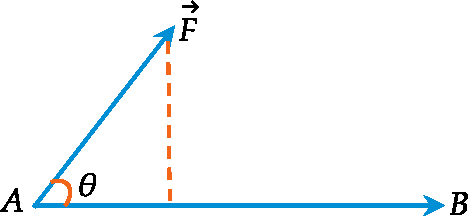
\includegraphics[width=0.85\textwidth]{workdone}
		\caption{Workdone in moving charge.}
	\end{figure}
\end{minipage}

\section{Electrostatic energy}
The work necessary to assemble a system of charges against coulomb forces is stored in the field as potential energy. This is known as electrostatic energy.
\subsection{Electrostatic energy of system of point charges}
Let us consider bringing point charges one by one, from far away.The first charge, $q_{1}$, takes no work, since there is no field yet to fight against. Bringing next charge $q_{2}$ cost a workdone. 
\begin{align}
\text{When $q_{2}$ }&\text{is placed work done}\\
W_{2}&=q_{2} V_{1}\\
\text{where $V_{1}$ }&\text{is the potential due to $q_{1}$ so,}\\
W_{2}&=\frac{1}{4 \pi \varepsilon_{0}} q_{2}\left(\frac{q_{1}}{R_{12}}\right)
\text{Similiarly,}\\
W_{3}&=\frac{1}{4 \pi \epsilon_{0}} q_{3}\left(\frac{q_{1}}{r_{13}}+\frac{q_{2}}{r_{23}}\right)\\
\text{Similarly, }&\text{the extra work to bring in $q_{4}$ will be}\\
W_{4}&=\frac{1}{4 \pi \epsilon_{0}} q_{4}\left(\frac{q_{1}}{r_{14}}+\frac{q_{2}}{r_{24}}+\frac{q_{3}}{r_{34}}\right) .\\
\text{The total work }&\text{necessary to assemble the first four charges, then, is}\\
W&=\frac{1}{4 \pi \epsilon_{0}}\left(\frac{q_{1} q_{2}}{r_{12}}+\frac{q_{1} q_{3}}{r_{13}}+\frac{q_{1} q_{4}}{r_{14}}+\frac{q_{2} q_{3}}{r_{23}}+\frac{q_{2} q_{4}}{r_{24}}+\frac{q_{3} q_{4}}{r_{34}}\right) .\\
\text{In general,}\\
W&=\frac{1}{4 \pi \varepsilon_{0}} \sum_{i=1}^{n} \sum_{j=1 \atop j>i}^{n} \frac{q_{i} q_{j}}{R_{i j}}=\frac{1}{8 \pi \varepsilon_{0}} \sum_{i=1}^{n} \sum_{j=1 \atop j \neq i}^{n} \frac{q_{i} q_{j}}{R_{i j}}\\
&=\frac{1}{2} \sum_{i=1}^{n} q_{i} V\left(r_{i}\right)\label{electrostatics energy
}
\end{align}
\begin{center}
	\framebox{
		\parbox[t][0.75cm]{4cm}{
			
			\addvspace{0.2cm} \centering 
			
			$ W= \frac{1}{2} \sum_{i=1}^{n} q_{i} V\left(r_{i}\right)$} }
\end{center}
Where $V\left(r_{i}\right)$ is the potential at point $r_{i}$ (the position of $q_{i}$ ) due to all other charges.
\begin{exercise}
	Four charges are situated at the corners of a square (side a ) as shown in figure. How much work does it take to assemble the whole configuration of four charges?
	\begin{figure}[H]
		\centering
		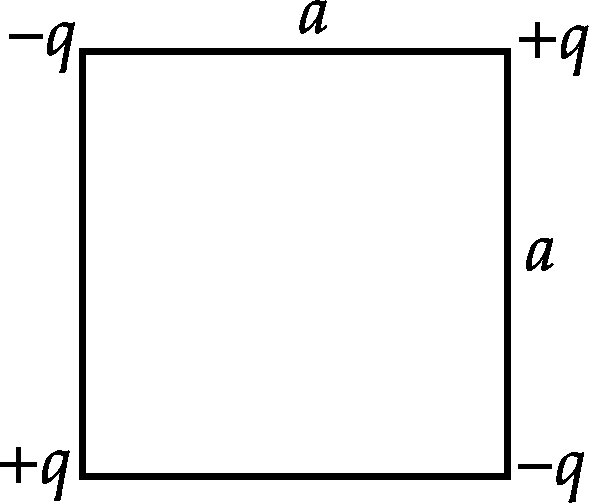
\includegraphics[height=3cm,width=4cm]{potential new}
	\end{figure}
\end{exercise}
\begin{answer}
	\begin{align*}
	\text{Work done in placing first charge ( $-q$ charge upper left corner) }W_{1}&=0\\
	\text{Work done in placing second charge ( $+q$ charge lower left corner)} W_{2}&=\frac{1}{4\pi \epsilon_{0}}\frac{-q^{2}}{a}\\
	\text{Work done in placing third charge ( $-q$ charge lower right corner)} W_{3}&=\frac{1}{4\pi \epsilon_{0}}\left( \frac{-q^{2}}{a}+\frac{-q^{2}}{\sqrt{2}a} \right) 
	\end{align*}
	Potential at fourth corner $(+q$ charge upper right corner $)$
	\begin{align*}
	V&=\frac{1}{4 \pi \varepsilon_{0}} \sum \frac{q_{i}}{r_{i}}=\frac{1}{4 \pi \varepsilon_{0}}\left(-\frac{q}{a}+\frac{q}{\sqrt{2} a}-\frac{q}{a}\right)\\&=\frac{q}{4 \pi \varepsilon_{0} a}\left(-2+\frac{1}{\sqrt{2}}\right) \\
	\Rightarrow W_{4}&=q V=\frac{q^{2}}{4 \pi \varepsilon_{0} a}\left(-2+\frac{1}{\sqrt{2}}\right) \\
	\text { Total work done }W&=W_{1}+W_{2}+W_{3}+W_{4}=\frac{1}{4 \pi \varepsilon_{0}} \frac{2 q^{2}}{a}\left(-2+\frac{1}{\sqrt{2}}\right)\\&=\frac{q^{2}}{2 \pi \varepsilon_{0} a}\left(-2+\frac{1}{\sqrt{2}}\right)
	\end{align*}
\end{answer}
\subsection{Energy of Continuous Charge Distribution}
For a system of volume charge density $\rho$ ,the equation \ref{electrostatics energy
} changes to,
\begin{equation}
W=\frac{1}{2} \int \rho V d \tau\label{continous charge}
\end{equation}
We know that,$(\vec{\nabla} \cdot \vec{E})=\frac{\rho}{\varepsilon_{0}}$
$\rightarrow$$\rho=\varepsilon_{0}(\vec{\nabla} \cdot \vec{E}) $ \\Then equation,\ \ref{continous charge} becomes,
\begin{align}
W&=\frac{\varepsilon_{0}}{2} \int(\vec{\nabla} \cdot \vec{E}) V d \tau\notag \\ W&=\frac{\varepsilon_{0}}{2}\left[-\int_{V} \vec{E} \cdot(\vec{\nabla} V) d \tau+\int_{V} \vec{\nabla} \cdot(V \vec{E}) d \tau\right]\notag\\
W&=\frac{\varepsilon_{0}}{2}\left[\int_{V} E^{2} d \tau+\oint_{S} V \vec{E} \cdot d \vec{a}\right] \hspace{1cm}\qquad\because\vec{E}=-\vec{\nabla} V \label{Electrostatic energy }
\end{align}
The above eq.\ref{Electrostatic energy } gives the correct energy $W$, whatever volume we use as long as it
encloses all the charges, but the contribution from the volume integral goes up, and that of
the surface integral goes down, as we take larger and larger volumes. In particular, if we
integrate over all space, then the surface integral goes to zero, and we have
$$
W=\frac{\varepsilon_{0}}{2} \int_{\text {all space }} E^{2} d \tau
$$
\subsubsection{Energy of uniformly charged spherical shell}
Consider a uniformly charged spherical shell of total charge $q$ and radius $R$.
\begin{align*}
\text{We know }&\text{that,}\\
\vec{E}_{\text {inside }}&=0, \quad \vec{E}_{\text {outside }}=\frac{1}{4 \pi \varepsilon_{0}} \frac{q}{r^{2}} \hat{r}\\
W&=\frac{\varepsilon_{0}}{2} \int_{\text {all space }} E^{2} d \tau\\&=\frac{\varepsilon_{0}}{2} \int_{0}^{R} E_{i n}^{2} d \tau+\frac{\varepsilon_{0}}{2} \int_{R}^{\infty} E_{\text {out }}^{2} d \tau\\&=\frac{\varepsilon_{0}}{2\left(4 \pi \varepsilon_{0}\right)^{2}} \int_{\text {outside }}\left(\frac{q^{2}}{r^{4}}\right)\left(r^{2} \sin \theta d r d \theta d \phi\right) \\
W&=\frac{1}{32 \pi^{2} \varepsilon_{0}} q^{2} 4 \pi \int_{R}^{\infty} \frac{1}{r^{2}} d r\\ W&=\frac{q^{2}}{8 \pi \varepsilon_{0} R}
\end{align*}
\subsubsection{Energy of uniformly charged solid sphere}
Consider a uniformly charged solid sphere of radius $R$ and charge $q$.
\begin{align*}
\text{We know}&\text{ that,}\\
\vec{E}&=\frac{1}{4 \pi \varepsilon_{0}} \frac{q r}{R^{3}} \hat{r}\quad ; \quad r>R \text {  and  } \vec{E}=\frac{1}{4 \pi \varepsilon_{0}} \frac{q}{r^{2}} \hat{r}\quad ; \quad r<R \\
W&=\frac{\varepsilon_{0}}{2} \frac{q^{2}}{\left(4 \pi \varepsilon_{0}\right)^{2}}\left\{\int_{R}^{\infty} \frac{1}{r^{4}}\left(r^{2} 4 \pi d r\right)+\int_{0}^{R}\left(\frac{r}{R^{3}}\right)^{2}\left(4 \pi r^{2} d r\right)\right\}\\&=\frac{1}{4 \pi \varepsilon_{0}} \frac{q^{2}}{2}\left\{\frac{1}{R}+\frac{1}{5 R}\right\} \\
W&=\frac{1}{20\pi \varepsilon_{0}} \frac{3 q^{2}}{ R}
\end{align*}
\newpage 
\begin{abox}
	The Method of Images
\end{abox}
\section{The Method of Images}
 The method of images concerns itself with the problem of one or more points charges in the presence of boundary surfaces, for example, conductors either grounded or held at fixed potentials. Under favorable conditons it is possible to infer from the geometry of the situation that a small number of suitably placed charges of appropriate magnitudes, exernal to tje reion of interest, can simulate the required boundary conditions. These charges are called image charges, and the replacement of the actual problem with boundaries by an enlarged region with image charges but not boundaries is called the method of images. The image charges must be external to the volume of interest, since their potentials must be solutions of the Laplace equation inside the volume; the "particular integral" (i.e.,solution of the poisson equation) is peovided by the sum of the potentials of the charges inside the volume.\\
A simple example is a point charge located in front of an infinite plane conductor at zero potential. 
\subsection{Point Charge in the Presence of a Grounded Conducting Sphere}
Suppose a point charge $q$ is held a distance $d$ above an infinite grounded conducting plane.$q$ will induce a certain amount of negative charge on the nearby surface of the conductor; the total potential is due in part to $q$ directly, and in part to this induced charge.\\
From a mathematical point of view, our problem is to solve Poisson's equation in the region $z>0$, with a single point charge $q$ at $(0,0, d)$, subject to the boundary conditions:\\
1. $V=0$ when $z=0$ (since the conducting plane is grounded), and\\
2. $V \rightarrow 0$ far from the charge (that is, for $x^{2}+y^{2}+z^{2} \gg d^{2}$ ).\\
The first uniqueness theorem (actually, its corollary) guarantees that there is only one function that meets these requirements.\\
Consider a new configuration consists of two point charges, $+q$ at \\\
\begin{figure}[H]
	\centering
	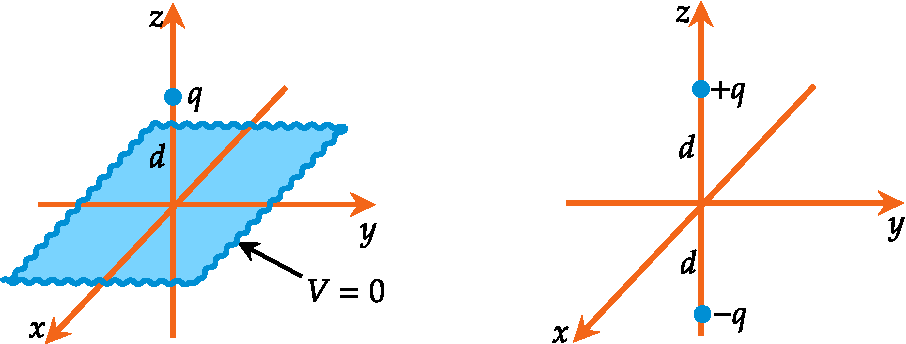
\includegraphics[height=3.5cm,width=9.5cm]{electric potential 02}
	\caption{}
	\label{}
\end{figure}
$(0,0, d)$ and $-q$ at $(0,0,-d)$, and no conducting plane . For this configuration, I can easily write down the potential:
\begin{equation}
V(x, y, z)=\frac{1}{4 \pi \epsilon_{0}}\left[\frac{q}{\sqrt{x^{2}+y^{2}+(z-d)^{2}}}-\frac{q}{\sqrt{x^{2}+y^{2}+(z+d)^{2}}}\right]\label{image charge 1}
\end{equation}

(The denominators represent the distances from $(x, y, z)$ to the charges $+q$ and $-q$, respectively.) It follows that\\
1. $V=0$ when $z=0$,\\
2. $V \rightarrow 0$ for $x^{2}+y^{2}+z^{2} \gg d^{2}$,\\
and the only charge in the region $z>0$ is the point charge $+q$ at $(0,0, d)$. But these are precisely the conditions of the original problem! Evidently the second configuration happens to produce exactly the same potential as the first configuration, in the "upper" region $z \geq 0 .$
\subsection{Induced Surface Charge}
\begin{align*}
\text{The surface charge $\sigma$ induced}&\text{ on the conductor.}\\
\sigma&=-\in_{0}\frac{\partial V}{\partial n}
\intertext{where $\partial V / \partial n$ is the normal derivative of $V$ at the surface. In this case the normal direction is the $z$ direction, so}
\sigma&=-\left.\epsilon_{0} \frac{\partial V}{\partial z}\right|_{z=0} .\\
\text{From Eq. \ref{image charge 1} ,}\\
\frac{\partial V}{\partial z}&=\frac{1}{4 \pi \epsilon_{0}}\left\{\frac{-q(z-d)}{\left[x^{2}+y^{2}+(z-d)^{2}\right]^{3 / 2}}+\frac{q(z+d)}{\left[x^{2}+y^{2}+(z+d)^{2}\right]^{3 / 2}}\right\}\\
\mathrm{so}\\
\sigma(x, y)&=\frac{-q d}{2 \pi\left(x^{2}+y^{2}+d^{2}\right)^{3 / 2}} .\\
\text{As expected, the induced }&\text{charge is negative (assuming $q$ is positive) and greatest at $x=y=0$.)}\\
\text{The total induced charge}\\
Q&=\int \sigma d a .
\intertext{This integral, over the $x y$ plane, could be done in Cartesian coordinates, with $d a=d x d y$, but it's a little easier to use polar coordinates $(r, \phi)$, with $r^{2}=x^{2}+y^{2}$ and $d a=r d r d \phi$. Then}
\sigma(r)&=\frac{-q d}{2 \pi\left(r^{2}+d^{2}\right)^{3 / 2}}\\
\text{ and }\quad
Q&=\int_{0}^{2 \pi} \int_{0}^{\infty} \frac{-q d}{2 \pi\left(r^{2}+d^{2}\right)^{3 / 2}} r d r d \phi=\left.\frac{q d}{\sqrt{r^{2}+d^{2}}}\right|_{0} ^{\infty}=-q .\\
\text{The total charge  }&\text{induced on the plane is $-q$}
\end{align*}





\subsection{Force and Energy}
The charge $q$ is attracted toward the plane, because of the negative induced charge. Let's calculate the force of attraction. Since the potential in the vicinity of $q$ is the same as in the analog problem (the one with $+q$ and $-q$ but no conductor), so also is the field and, therefore, the force:
\begin{align*}
\mathbf{F}&=-\frac{1}{4 \pi \epsilon_{0}} \frac{q^{2}}{(2 d)^{2}} \hat{\mathbf{z}} \\
\text{Think of the energy }&\text{stored in the fields:}\\
W&=\frac{\epsilon_{0}}{2} \int E^{2} d \tau .
\end{align*}
In the first case, both the upper region $(z>0)$ and the lower region $(z<0)$ contribute-and by symmetry they contribute equally. But in the second case, only the upper region contains a nonzero field, and hence the energy is half as great.\\
For a single charge and conducting plane, the energy is half of energy due to two point charges
\begin{align*}
W&=-\frac{1}{4 \pi \epsilon_{0}} \frac{q^{2}}{4 d}\\
\text{work }&\text{required to bring $g$ in from infinity}\\
W &=\int_{\infty}^{d} \mathbf{F} \cdot d \mathbf{l}=\frac{1}{4 \pi \epsilon_{0}} \int_{\infty}^{d} \frac{q^{2}}{4 z^{2}} d z \\
&=\left.\frac{1}{4 \pi \epsilon_{0}}\left(-\frac{q^{2}}{4 z}\right)\right|_{\infty} ^{d}=-\frac{1}{4 \pi \epsilon_{0}} \frac{q^{2}}{4 d} .
\end{align*}
\newpage 
\begin{abox}
	Multipole Expansion
\end{abox}
\section{Multipole Expansion}
If you are very far away from a localized charge distribution, it "looks" like a point charge,and the potential is
$$V=\frac{1}{4\pi \varepsilon_{0}}\frac{Q}{r}$$
Where $Q$ is the total charge\\\\
But what if $Q$ is zero?
\subsection{Electric Dipole}
 A physical electric dipole consists of two equal and opposite charges $(\pm q)$ seperated by a distance $d$. 
\begin{figure}[H]
	\centering
	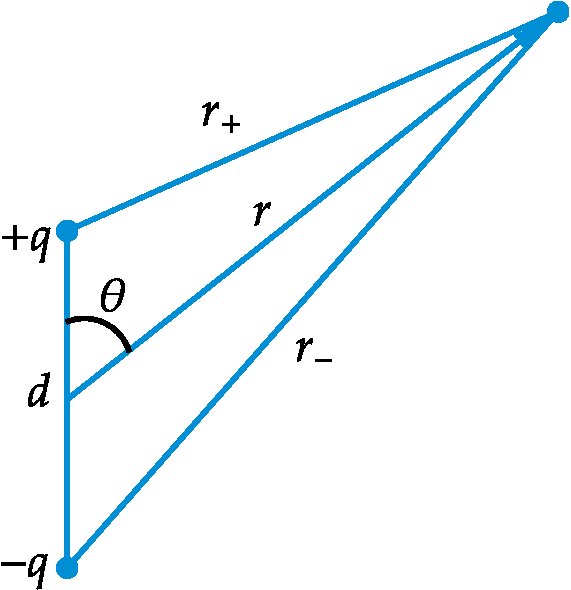
\includegraphics[height=4cm,width=4cm]{electric potential 17}
	\caption{}
	\label{}
\end{figure}
\begin{align*}
\text{Let $r_{-}$be the distance from $-q$}&\text{  and $r_{+}$the distance from $+q$ (Fig. 26). Then}\\
V(\mathbf{r})&\approx\frac{1}{4 \pi \epsilon_{0}}\left(\frac{q}{r_{+}}-\frac{q}{r_{-}}\right),\\
\text{and (from the law of cosines)}\\
r_{\pm}^{2}&=r^{2}+(d / 2)^{2} \mp r d \cos \theta=r^{2}\left(1 \mp \frac{d}{r} \cos \theta+\frac{d^{2}}{4 r^{2}}\right) .\\
\text{We're interested in the régime}&\text{ $r \gg d$, so the third term is negligible, and the binomial expansion yields}\\
\frac{1}{r_{\pm}} &\cong \frac{1}{r}\left(1 \mp \frac{d}{r} \cos \theta\right)^{-1 / 2} \cong \frac{1}{r}\left(1 \pm \frac{d}{2 r} \cos \theta\right) \text {. }\\
\text{Thus}\quad
\frac{1}{r_{+}}-\frac{1}{r_{-}} &\cong \frac{d}{r^{2}} \cos \theta,\\
\text{and hence}\quad
V(\mathbf{r}) &\cong \frac{1}{4 \pi \epsilon_{0}} \frac{q d \cos \theta}{r^{2}}
\end{align*}
The potential of a dipole goes like $1 / r^{2}$ at large $r$; as we might have anticipated, it falls off more rapidly than the potential of a point charge. If we put together a pair of equal and opposite dipoles to make a quadrupole, the potential goes like $1 / r^{3}$; for back-to-back quadrupoles (an octopole), it goes like $1 / r^{4}$; and so on. Figure 27 summarizes this hierarchy; for completeness I have included the electric monopole (point charge), whose potential, of course, goes like $1 / r$.
\begin{figure}[H]
	\begin{minipage}{0.24\textwidth}
		
\includegraphics[width=0.25\textwidth]{monopole}
		\caption{Monopole}
	\end{minipage}
	\begin{minipage}{0.24\textwidth}
		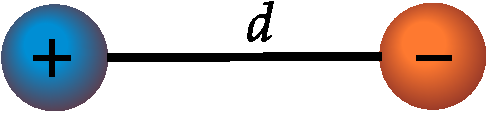
\includegraphics[width=0.65\textwidth]{dipole}
		\caption{Dipole}
	\end{minipage}
	\begin{minipage}{0.24\textwidth}
		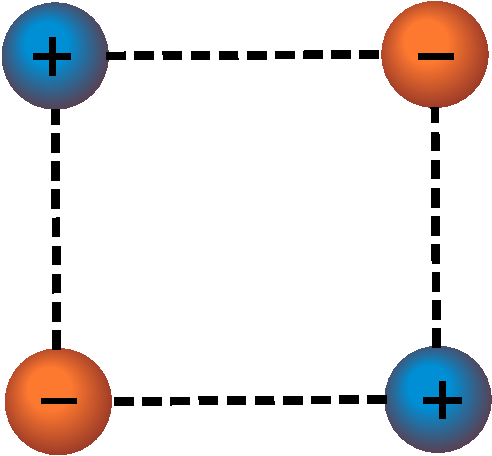
\includegraphics[width=0.65\textwidth]{quadrapole}
		\caption{Quadrapole}
	\end{minipage}
	\begin{minipage}{0.24\textwidth}
		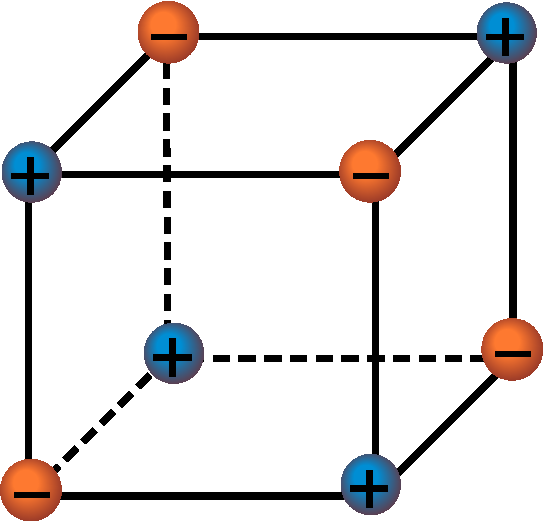
\includegraphics[width=0.65\textwidth]{octapole}
		\caption{Octapole}
	\end{minipage}
\end{figure}
To develop a systematic expansion for the potential of any localized charge distribution, in powers of $1/r$, the potential at $r$ is given by \\
\begin{figure}[H]
	\centering
	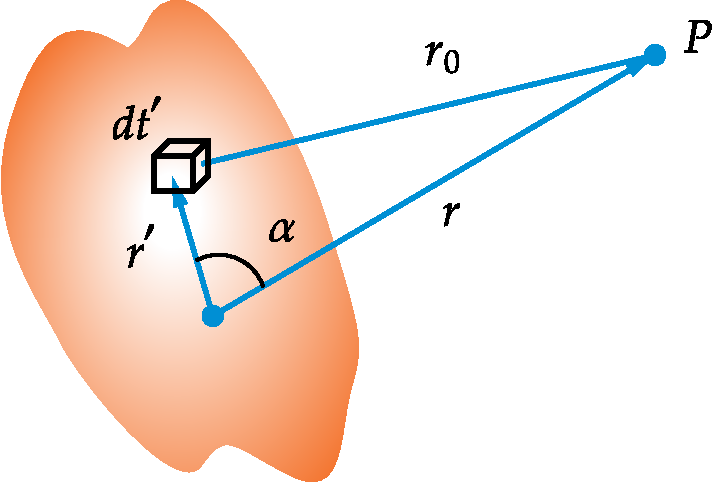
\includegraphics[height=3.5cm,width=6cm]{Electric potential 19}
	\caption{}
	\label{}
\end{figure}
\begin{equation}
V(\mathbf{r})=\frac{1}{4 \pi \epsilon_{0}} \int \frac{1}{r_0} \rho\left(\mathbf{r}^{\prime}\right) d \tau^{\prime}\label{EP1}
\end{equation}
\begin{align*}
\text{Using the law of }&\text{cosines,}\\
r_0^{2}&=r^{2}+\left(r^{\prime}\right)^{2}-2 r r^{\prime} \cos \alpha\\
&=r^{2}\left[1+\left(\frac{r^{\prime}}{r}\right)^{2}-2\left(\frac{r^{\prime}}{r}\right) \cos \alpha\right]\\
\text{where $\alpha$ is the angle}&\text{ between $\mathbf{r}$ and $\mathbf{r}^{\prime}$. Thus}\\
r_0&=r \sqrt{1+\epsilon}\\
\text{with, }&\varepsilon \equiv\left(\frac{r^{\prime}}{r}\right)\left(\frac{r^{\prime}}{r}-2 \cos \alpha\right)\\
\text{For points well outside the charge }&\text{distribution, $\epsilon$ is much less than 1 , and this invites a binomial expansion:}\\
\frac{1}{r_0}&=\frac{1}{r}(1+\epsilon)^{-1 / 2}\\
&=\frac{1}{r}\left(1-\frac{1}{2} \epsilon+\frac{3}{8} \epsilon^{2}-\frac{5}{16} \epsilon^{3}+\ldots\right)\\
\text{or, in terms of }&\text{$r, r^{\prime}$, and $\alpha$ :}\\
\frac{1}{r_0}&=\frac{1}{r}\left[1-\frac{1}{2}\left(\frac{r^{\prime}}{r}\right)\left(\frac{r^{\prime}}{r}-2 \cos \alpha\right)+\frac{3}{8}\left(\frac{r^{\prime}}{r}\right)^{2}\left(\frac{r^{\prime}}{r}-2 \cos \alpha\right)^{2}\right. \\
& \left. \right.  \quad \left.-\frac{5}{16}\left(\frac{r^{\prime}}{r}\right)^{3}\left(\frac{r^{\prime}}{r}-2 \cos \alpha\right)^{3}+\ldots\right] \\
&=\frac{1}{r}\left[1+\left(\frac{r^{\prime}}{r}\right)(\cos \alpha)+\left(\frac{r^{\prime}}{r}\right)^{2}\left(\frac{3 \cos ^{2} \alpha-1}{2}\right)\right. \\
\left. \right.  \quad &\left.+\left(\frac{r^{\prime}}{r}\right)^{3}\left(\frac{5 \cos ^{3} \alpha-3 \cos \alpha}{2}\right)+\ldots\right]
\end{align*}
\begin{align*}
\text{Here it is collected together like powers}&\text{  of $(r^\prime/r)$ and their coefficients are Legendre polynomials.So, }\\
\frac{1}{r}&=\frac{1}{r} \sum_{n=0}^{\infty}\left(\frac{r^{\prime}}{r}\right)^{n} P_{n}(\cos \alpha) \\
\text{Substituting this back into Eq. \ref{EP1} , and   }&\text{noting that $r$ is a constant, as far as the integration is concerned, We get}\\
V(\mathbf{r})&=\frac{1}{4 \pi \epsilon_{0}} \sum_{n=0}^{\infty} \frac{1}{r^{(n+1)}} \int\left(r^{\prime}\right)^{n} P_{n}(\cos \alpha) \rho\left(\mathbf{r}^{\prime}\right) d \tau^{\prime}\\
\text{or, more explicitly,}\\
V(\mathbf{r})&=\frac{1}{4 \pi \epsilon_{0}}\left[  \frac{1}{r} \int \rho\left(\mathbf{r}^{\prime}\right) d \tau^{\prime}+\frac{1}{r^{2}} \int r^{\prime} \cos \alpha \rho\left(\mathbf{r}^{\prime}\right) d \tau^{\prime}\right.  \\
&\left.+\frac{1}{r^{3}} \int\left(r^{\prime}\right)^{2}\left(\frac{3}{2} \cos ^{2} \alpha-\frac{1}{2}\right) \rho\left(\mathbf{r}^{\prime}\right) d \tau^{\prime}+\ldots\right] \\
\text{This is the desired result}&\text{-the multipole expansion of $V$ in powers of $1/r$.}
\end{align*}
\textbf{Monopole Term}
\begin{itemize}
	\item The first term $(n=0)$ is the monopole contribution (it goes like $1 / r)$
\item	Ordinarily, the multipole expansion is dominated (at large $r$ ) by the monopole term:
	$$
	V_{\text {mon }}(\mathbf{r})=\frac{1}{4 \pi \epsilon_{0}} \frac{Q}{r},
	$$
	where $Q=\int \rho d \tau$ is the total charge of the configuration.
\end{itemize}
\textbf{Dipole Term}
\begin{itemize}
	\item The second $(n=1)$ is the dipole (it goes like $\left.1 / r^{2}\right)$
\end{itemize}
If the total charge is zero, the dominant term in the potential will be the dipole (unless it also vanishes):
\begin{align*}
V_{\mathrm{dip}}(\mathbf{r})&=\frac{1}{4 \pi \epsilon_{0}} \frac{1}{r^{2}} \int r^{\prime} \cos \alpha \rho\left(\mathbf{r}^{\prime}\right) d \tau^{\prime} .\\
\text{Since $\alpha$ is the angle between }&\text{$\mathbf{r}^{\prime}$ and $\mathbf{r}$ ,}\\
r^{\prime} \cos \alpha&=\hat{\mathbf{r}} \cdot \mathbf{r}^{\prime},\\
\text{and the dipole potential can}&\text{ be written as:}\\
V_{\text {dip }}(\mathbf{r})&=\frac{1}{4 \pi \epsilon_{0}} \frac{1}{r^{2}} \hat{\mathbf{r}} \cdot \int \mathbf{r}^{\prime} \rho\left(\mathbf{r}^{\prime}\right) d \tau^{\prime} .\\
\text{This integral (which does not depend on}&\text{ $\mathbf{r}$ ) is called the dipole moment of the distribution:}\\
\mathbf{p} &\equiv \int \mathbf{r}^{\prime} \rho\left(\mathbf{r}^{\prime}\right) d \tau^{\prime}\\
\text{and the dipole contribution }&\text{to the potential simplifies to}\\
V_{\text {dip }}(\mathbf{r})&=\frac{1}{4 \pi \epsilon_{0}} \frac{\mathbf{p} \cdot \hat{\mathbf{r}}}{r^{2}}\\
\text{The dipole moment is determined }&\text{by the geometry of the charge distribution.}\\
\text{ Dipole moment of a collection }&\text{of point charges is}\\
\mathbf{p}&=\sum_{i=1}^{n} q_{i} \mathbf{r}_{i}^{\prime} .
\end{align*}
\begin{note}
	The third is quadrupole,the fourth octopole and so on. Remember that $\alpha$ is the angle between $\mathbf{r}$ and $\mathbf{r}^{\prime}$, so the integrals depend on the direction to the field point.
\end{note}
\section{Potential energy of a dipole placed in an external electric field}
Let we put a dipole whose $-q$ and $+$ q respectively at $\vec{r}$ and $(\vec{r}+\vec{d})$
The potential energy,
\begin{align*}
U&=-q V(\vec{r})+q V(\vec{r}+\vec{d})\\
U&=-q V(r)+q V(r)+q d \cdot \vec{\nabla} V(r)\quad \text{(using Taylor expansion)}\\
&=q d \cdot \vec{\nabla} V(r) \\
U&=\vec{p} \cdot \vec{\nabla} V(r) \\
U&=-\vec{p} \cdot \vec{E}(r) \quad(\because E(r)=-\nabla V(r))
\end{align*}
\subsection{Force and torque on a dipole placed in an electric field:}
\subsubsection{Force }
\begin{align*}
\text{We  }&\text{know that,}\\
\vec{F} &=-\vec{\nabla} U=\nabla(\vec{p} \cdot \vec{E}) \\
&=(\vec{p} \cdot \vec{\nabla}) \vec{E}+(\vec{E} \cdot \vec{\nabla}) \vec{p}+\vec{p} \times(\vec{\nabla} \times \vec{E})+\vec{E} \times(\vec{\nabla} \times \vec{p}) \\
&=(\vec{p} \cdot \vec{\nabla}) \bar{E}+0+0+0\\
\text{For } &\text{uniform }\vec{E},\\
\vec{F}&=(\vec{p} \cdot \vec{\nabla}) \vec{E}=0
\end{align*}

that means there have no translational motion.
\subsubsection{Torque}
We know the potential energy of the dipole due external electrie field is $u=\vec{p} \cdot \vec{E}=p E \cos \theta$
Therefore, the torque about its own centre is
$$
\begin{aligned}
\tau&=-\frac{d u}{d \theta}=p E \sin \theta\\
&\text { Or, }\\
\vec{\tau}&=\vec{p} \times \vec{E}
\end{aligned}
$$
\textbf{Torque on the dipole in non-uniform electric field :}\\
The torque on a small dipole about its own centre is still
$$
\vec{\tau}=\vec{p} \times \vec{E}
$$
But since there is a net force $\vec{F}$ on the dipole.
Therefore, an extra torque act on the dipole is $\vec{r} \times \vec{F}$ about any other point.
Therefore, totaltorque about any other point is $\vec{\tau}=\vec{p} \times \vec{E}+\vec{r} \times \vec{F}$\\
\textbf{Mutual potential energy between two coplanar dipoles:}\\
Let consider two diple of dipole moment $\vec{p}_{1}$ and $\vec{p}_{2}$ lying on a single plane, $\vec{r}_{21}$ is the position vector of dipole
2 with respect to 1 . The electric field at the centre of dipole 2 is,
\begin{align*}
\vec{E}_{1}&=\frac{1}{4 \pi \varepsilon_{0}}\left[\frac{3\left(\vec{p}_{1} \cdot \vec{r}_{21}\right) \vec{r}_{21}}{r_{21}^{5}}-\frac{\vec{p}_{1}}{r_{21}^{3}}\right]\\
\text{The mutual}&\text{ potential energy,}\\
U_{21}&=-\vec{p}_{2} \cdot \vec{E}_{1}=-\vec{p}_{1} \cdot \vec{E}_{2}\\&=\frac{1}{4 \pi \varepsilon_{0}}\left[\frac{\vec{p}_{1} \cdot \vec{p}_{2}}{r_{21}^{3}}-\frac{3\left(\vec{p}_{1} \cdot \vec{r}_{21}\right)\left(\vec{p}_{2} \cdot \vec{r}_{21}\right)}{r_{21}^{5}}\right]
\end{align*}



 
\newpage
\begin{abox}
	Practise Set-1
	\end{abox}
\begin{enumerate}[label=\color{ocre}\textbf{\arabic*.}]
	\item  The electrostatic potential $V(x, y)$ in free space in a region where the charge density $\rho$ is zero is given by $V(x, y)=4 e^{2 x}+f(x)-3 y^{2}$. Given that the $x$-component of the electric field $E_{x}$, and $V$ are zero at the origin, $f(x)$ is
	{\exyear{ NET/JRF(JUNE-2011)}}
	\begin{tasks}(2)
		\task[\textbf{A.}] $3 x^{2}-4 e^{2 x}+8 x$
		\task[\textbf{B.}] $3 x^{2}-4 e^{2 x}+16 x$
		\task[\textbf{C.}] $4 e^{2 x}-8$
		\task[\textbf{D.}] $3 x^{2}-4 e^{2 x}$
	\end{tasks}
	\item A static, spherically symmetric charge distribution is given by $\rho(r)=\frac{A}{r} e^{-K r}$ where $A$ and $K$ are positive constants. The electrostatic potential corresponding to this charge distribution varies with $r$ as
	{\exyear{NET/JRF(JUNE-2011)}}
	\begin{tasks}(4)
		\task[\textbf{A.}] $r e^{-K r}$
		\task[\textbf{B.}] $\frac{1}{r} e^{-K r}$
		\task[\textbf{C.}] $\frac{1}{r^{2}} e^{-K r}$
		\task[\textbf{D.}] $\frac{1}{r}\left(1-e^{-K r}\right)$
	\end{tasks}
	\item Charges $Q, Q$ and $-2 Q$ are placed on the vertices of an equilateral triangle $A B C$ of sides of length $a$, as shown in the figure. The dipole moment of this configuration of charges, irrespective of the choice of origin, is
	{\exyear{NET/JRF(JUNE-2012)}}
	\begin{figure}[H]
		\centering
		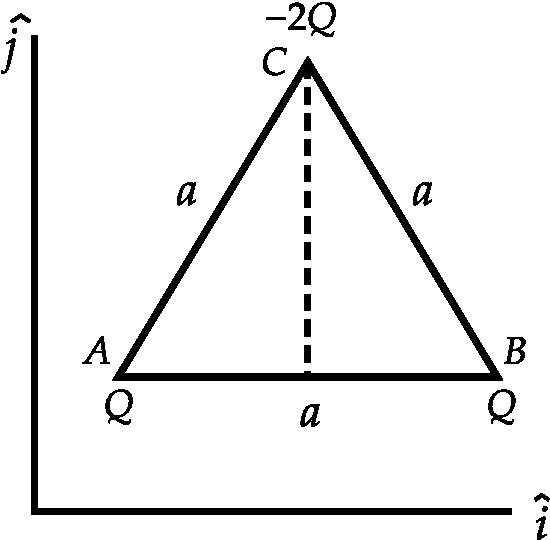
\includegraphics[height=4.5cm,width=4cm]{Electric potential 03}
		\caption{}
		\label{}
	\end{figure}
	\begin{tasks}(4)
		\task[\textbf{A.}] $+2 a Q \hat{i}$
		\task[\textbf{B.}] $+\sqrt{3} a Q \hat{j}$
		\task[\textbf{C.}] $-\sqrt{3} a Q \hat{j}$
		\task[\textbf{D.}] 0
	\end{tasks}
	\item  Four charges (two $+q$ and two $-q$ ) are kept fixed at the four vertices of a square of side $a$ as shown. At the point $P$ which is at a distance $R$ from the centre $(R>>a)$, the potential is proportional to
	{\exyear{NET/JRF(DEC-2012)}}
	\begin{figure}[H]
		\centering
		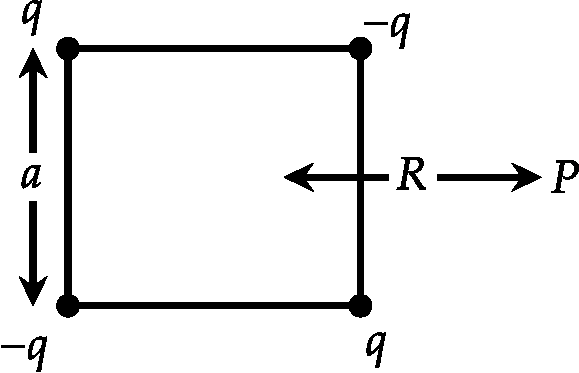
\includegraphics[height=3cm,width=4.2cm]{electric potential 04}
	\end{figure}
	\begin{tasks}(4)
		\task[\textbf{A.}] $1 / R$
		\task[\textbf{B.}] $1 / R^{2}$
		\task[\textbf{C.}] $1 / R^{3}$
		\task[\textbf{D.}] $1 / R^{4}$
	\end{tasks}
	\item  A point charges $q$ of mass $m$ is kept at a distance $d$ below a grounded infinite conducting sheet which lies in the $x y$ - plane. For what value of $d$ will the charge remains stationary?
	{\exyear{NET/JRF(DEC-2012)}}
	\begin{tasks}(2)
		\task[\textbf{A.}] $q / 4 \sqrt{m g \pi \varepsilon_{0}}$
		\task[\textbf{B.}] $q / \sqrt{m g \pi \varepsilon_{0}}$
		\task[\textbf{C.}] There is no finite value of $d$
		\task[\textbf{D.}]  $\sqrt{m g \pi \varepsilon_{0}} / q$
	\end{tasks}
	\item A particle of charge $e$ and mass $m$ is located at the midpoint of the line joining two fixed collinear dipoles with unit charges as shown in the figure. (The particle is constrained to move only along the line joining the dipoles). Assuming that the length of the dipoles is much shorter than their separation, the natural frequency of oscillation of the particle is
	{\exyear{NET/JRF(JUNE-2013)}}
	\begin{figure}[H]
		\centering
		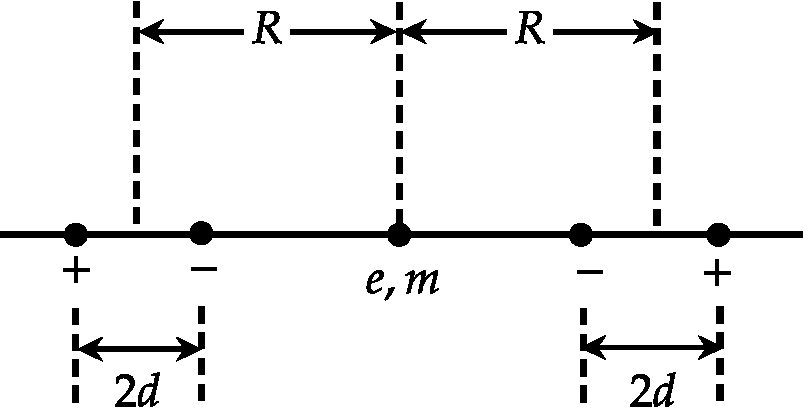
\includegraphics[height=3.5cm,width=7cm]{electric potential 05}
	\end{figure}
	\begin{tasks}(4)
		\task[\textbf{A.}] $\sqrt{\frac{6 e R^{2}}{\pi \varepsilon_{0} m d^{5}}}$
		\task[\textbf{B.}] $\sqrt{\frac{6 e R}{\pi \varepsilon_{0} m d^{4}}}$
		\task[\textbf{C.}]  $\sqrt{\frac{6 e d^{2}}{\pi \varepsilon_{0} m R^{5}}}$
		\task[\textbf{D.}] $\sqrt{\frac{6 e d}{\pi \varepsilon_{0} m R^{4}}}$
	\end{tasks}
	\item Consider an axially symmetric static charge distribution of the form,
	$$
	\rho=\rho_{0}\left(\frac{r_{0}}{r}\right)^{2} e^{-r / r_{0}} \cos ^{2} \varphi
	$$
	The radial component of the dipole moment due to this charge distribution is
	{\exyear{NET/JRF(JUNE-2013)}}
	\begin{tasks}(4)
		\task[\textbf{A.}] $2 \pi \rho_{0} r_{0}^{4}$
		\task[\textbf{B.}] $\pi \rho_{0} r_{0}^{4}$
		\task[\textbf{C.}] $\rho_{0} r_{0}^{4}$
		\task[\textbf{D.}] $\pi \rho_{0} r_{0}^{4} / 2$
	\end{tasks}
	\item A point charge $q$ is placed symmetrically at a distance $d$ from two perpendicularly placed grounded conducting infinite plates as shown in the figure. The net force on the charge (in units of $1 / 4 \pi \varepsilon_{0}$ ) is
	{\exyear{NET/JRF(DEC-2013)}}
	\begin{figure}[H]
		\centering
		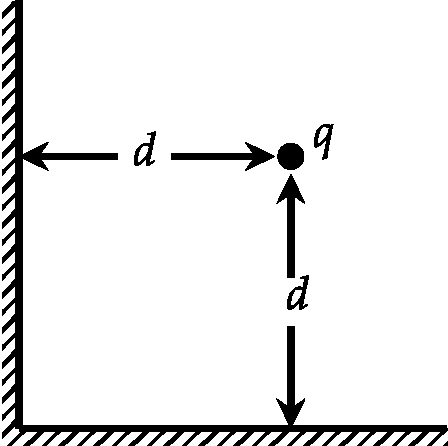
\includegraphics[height=4.5cm,width=5cm]{electric potential 07}
	\end{figure}
	\begin{tasks}(2)
		\task[\textbf{A.}] $\frac{q^{2}}{8 d^{2}}(2 \sqrt{2}-1)$ away from the corner
		\task[\textbf{B.}] $\frac{q^{2}}{8 d^{2}}(2 \sqrt{2}-1)$ towards the corner
		\task[\textbf{C.}] $\frac{q^{2}}{2 \sqrt{2} d^{2}}$ towards the corner
		\task[\textbf{D.}] $\frac{3 q^{2}}{8 d^{2}}$ away from the corner
	\end{tasks}
	\item If the electrostatic potential $V(r, \theta, \phi)$ in a charge free region has the form $V(r, \theta, \phi)=f(r) \cos \theta$, then the functional form of $f(r)$ (in the following $a$ and $b$ are constants) is:
	{\exyear{NET/JRF(DEC-2013)}}
	\begin{tasks}(4)
		\task[\textbf{A.}] $a r^{2}+\frac{b}{r}$
		\task[\textbf{B.}] $a r+\frac{b}{r^{2}}$
		\task[\textbf{C.}] $a r+\frac{b}{r}$
		\task[\textbf{D.}] $a \ln \left(\frac{r}{b}\right)$
	\end{tasks}
	\item  Let four point charges $q,-q / 2, q$ and $-q / 2$ be placed at the vertices of a square of side $a$. Let another point charge $-q$ be placed at the centre of the square (see the figure).\\
	\begin{figure}[H]
		\centering
		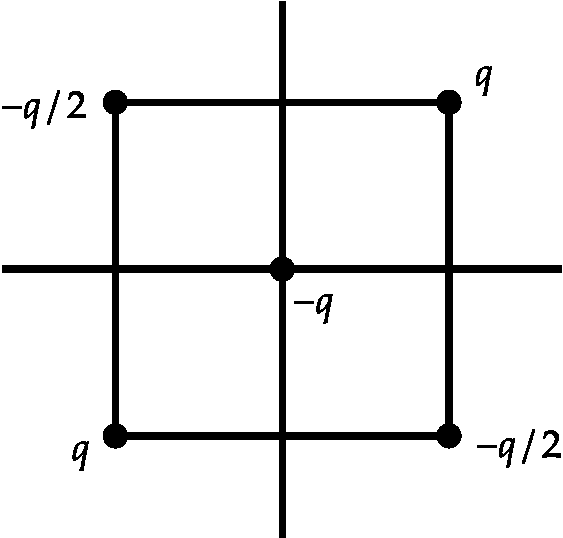
\includegraphics[height=4.5cm,width=5cm]{electric potential 09}
	\end{figure}
	Let $V(r)$ be the electrostatic potential at a point $P$ at a distance $r>>a$ from the centre of the square. Then $V(2 r) / V(r)$ is
	{\exyear{NET/JRF(DEC-2013)}}
	\begin{tasks}(4)
		\task[\textbf{A.}] 1
		\task[\textbf{B.}]  $\frac{1}{2}$
		\task[\textbf{C.}] $\frac{1}{4}$
		\task[\textbf{D.}] $\frac{1}{8}$
	\end{tasks}
	\item If the electrostatic potential in spherical polar coordinates is
	$$
	\varphi(r)=\varphi_{0} e^{-r / r_{0}}
	$$
	where $\varphi_{0}$ and $r_{0}$ are constants, then the charge density at a distance $r=r_{0}$ will be
	{\exyear{NET/JRF(JUNE-2014)}}
	\begin{tasks}(4)
		\task[\textbf{A.}] $\frac{\varepsilon_{0} \varphi_{0}}{e r_{0}^{2}}$
		\task[\textbf{B.}] $\frac{e \varepsilon_{0} \varphi_{0}}{2 r_{0}^{2}}$
		\task[\textbf{C.}] $-\frac{\varepsilon_{0} \varphi_{0}}{e r_{0}^{2}}$
		\task[\textbf{D.}] $-\frac{2 e \varepsilon_{0} \varphi_{0}}{r_{0}^{2}}$
	\end{tasks}
	\item A charge $(-e)$ is placed in vacuum at the point $(d, 0,0)$, where $d>0 .$ The region $x \leq 0$ is filled uniformly with a metal. The electric field at the point $\left(\frac{d}{2}, 0,0\right)$ is
	{\exyear{NET/JRF(JUNE-2014)}}
	\begin{tasks}(2)
		\task[\textbf{A.}]  $-\frac{10 e}{9 \pi \varepsilon_{0} d^{2}}(1,0,0)$
		\task[\textbf{B.}]  $\frac{10 e}{9 \pi \varepsilon_{0} d^{2}}(1,0,0)$
		\task[\textbf{C.}] $\frac{e}{\pi \varepsilon_{0} d^{2}}(1,0,0)$
		\task[\textbf{D.}] $-\frac{e}{\pi \varepsilon_{0} d^{2}}(1,0,0)$
	\end{tasks}
\item A charged particle is at a distance $d$ from an infinite conducting plane maintained at zero potential. When released from rest, the particle reaches a speed $u$ at a distance $d / 2$ from the plane. At what distance from the plane will the particle reach the speed $2 u ?$
{\exyear{NET/JRF(JUNE-2014)}}
\begin{tasks}(4)
	\task[\textbf{A.}] $d / 6$
	\task[\textbf{B.}] $d / 3$
	\task[\textbf{C.}] $d / 4$
	\task[\textbf{D.}] $d / 5$
\end{tasks}
\item  The electrostatic lines of force due to a system of four point charges is sketched here. At large distance $r$, the leading asymptotic behaviour of the electrostatic potential is proportional to
{\exyear{NET/JRF(DEC-2014)}}
\begin{figure}[H]
	\centering
	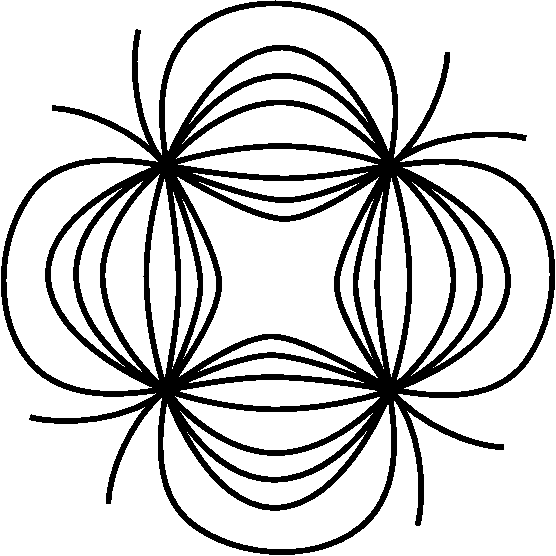
\includegraphics[height=4.5cm,width=4cm]{electric potential 12}
\end{figure}
\begin{tasks}(4)
	\task[\textbf{A.}] $r$
	\task[\textbf{B.}] $r^{-1}$
	\task[\textbf{C.}] $r^{-2}$
	\task[\textbf{D.}] $r^{-3}$
\end{tasks}
\item A hollow metallic sphere of radius $a$, which is kept at a potential $V_{0}$ has a charge $Q$ at its centre. The potential at a point outside the sphere, at a distance $r$ from the centre, is
{\exyear{NET/JRF(DEC-2015)}}
\begin{tasks}(4)
	\task[\textbf{A.}] $V_{0}$
	\task[\textbf{B.}] $\frac{Q}{4 \pi \in_{0} r}+\frac{V_{0} a}{r}$
	\task[\textbf{C.}] $\frac{Q}{4 \pi \in_{0} r}+\frac{V_{0} a^{2}}{r^{2}}$
	\task[\textbf{D.}] $\frac{V_{0} a}{r}$
\end{tasks}
\item Two uniformly charged insulating solid spheres $A$ and $B$, both of radius $a$, carry total charges $+Q$ and $-Q$, respectively. The spheres are placed touching each other as shown in the figure.\\
\begin{figure}[H]
	\centering
	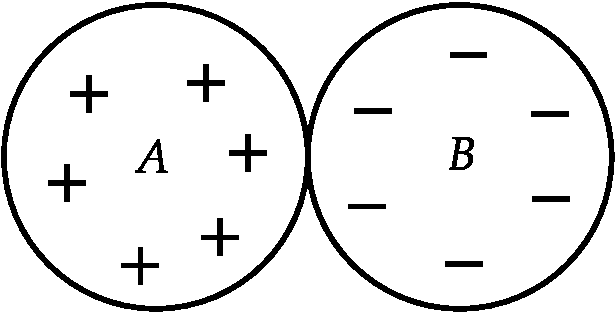
\includegraphics[height=2.5cm,width=4.7cm]{diagram-20211011(50)-crop}
\end{figure}
If the potential at the centre of the sphere $A$ is $V_{A}$ and that at the centre of $B$ is $V_{B}$ then the difference $V_{A}-V_{B}$ is
{\exyear{NET/JRF(DEC-2016)}}
\begin{tasks}(4)
	\task[\textbf{A.}] $\frac{Q}{4 \pi \varepsilon_{0} a}$
	\task[\textbf{B.}] $\frac{-Q}{2 \pi \varepsilon_{0} a}$
	\task[\textbf{C.}] $\frac{Q}{2 \pi \varepsilon_{0} a}$
	\task[\textbf{D.}] $\frac{-Q}{4 \pi \varepsilon_{0} a}$
\end{tasks}
\item Two long hollow co-axial conducting cylinders of radii $R_{1}$ and $R_{2}\left(R_{1}<R_{2}\right)$ are placed in vacuum as shown in the figure below.\\
\begin{figure}[H]
	\centering
	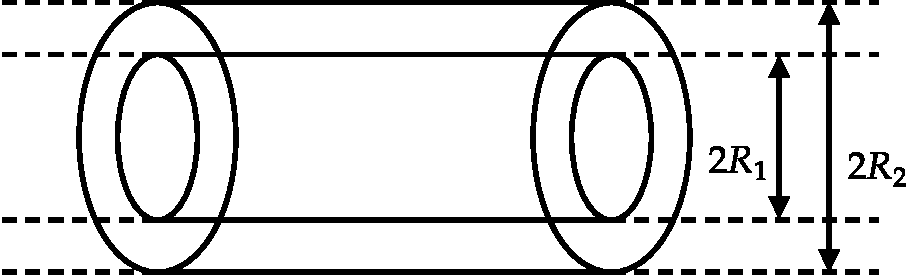
\includegraphics[height=2.5cm,width=7.5cm]{electric potential 13}
\end{figure}
The inner cylinder carries a charge $+\lambda$ per unit length and the outer cylinder carries a charge $-\lambda$ per unit length. The electrostatic energy per unit length of this system is
{\exyear{NET/JRF(JUNE-2017)}}
\begin{tasks}(2)
	\task[\textbf{A.}] $\frac{\lambda^{2}}{\pi \in_{0}} \ln \left(R_{2} / R_{1}\right)$
	\task[\textbf{B.}] $\frac{\lambda^{2}}{4 \pi \epsilon_{0}}\left(R_{2}^{2} / R_{1}^{2}\right)$
	\task[\textbf{C.}] $\frac{\lambda^{2}}{4 \pi \epsilon_{0}} \ln \left(R_{2} / R_{1}\right)$
	\task[\textbf{D.}] $\frac{\lambda^{2}}{2 \pi \epsilon_{0}} \ln \left(R_{2} / R_{1}\right)$
\end{tasks}
\item Two point charges $+3 Q$ and $-Q$ are placed at $(0,0, d)$ and $(0,0,2 d)$ respectively, above an infinite grounded conducting sheet kept in the $x y$ - plane. At a point $(0,0, z)$, where $z>>d$, the electrostatic potential of this charge configuration would approximately be
{\exyear{NET/JRF(DEC-2017)}}
\begin{tasks}(4)
	\task[\textbf{A.}] $\frac{1}{4 \pi \varepsilon_{0}} \frac{d^{2}}{z^{3}} Q$
	\task[\textbf{B.}] $\frac{1}{4 \pi \varepsilon_{0}} \frac{2 d}{z^{2}} Q$
	\task[\textbf{C.}] $\frac{1}{4 \pi \varepsilon_{0}} \frac{3 d}{z^{2}} Q$
	\task[\textbf{D.}] $-\frac{1}{4 \pi \varepsilon_{0}} \frac{d^{2}}{z^{3}} Q$
\end{tasks}
\item  Two point charges $+2 Q$ and $-Q$ are kept at point with Cartesian coordinates $(1,0,0)$, respectively, in front of an infinite grounded conducting plate at $x=0$. The potential at $(x, 0,0)$ for $x \gg 1$ depends on $x$ as
{\exyear{NET/JRF(JUNE-2018)}}
\begin{tasks}(4)
	\task[\textbf{A.}] $x^{-3}$
	\task[\textbf{B.}]  $x^{-5}$
	\task[\textbf{C.}] $x^{-2}$
	\task[\textbf{D.}] $x^{-4}$
\end{tasks}
\item An electric dipole of dipole moment $\vec{P}=q b \hat{i}$ is placed at origin in the vicinity of two charges $+q$ and $-q$ at $(L, b)$ and $(L,-b)$, respectively, as shown in the figure. The electrostatic potential at the point $\left(\frac{L}{2}, 0\right)$ is
{\exyear{NET/JRF(DEC-2018)}}
\begin{figure}[H]
	\centering
	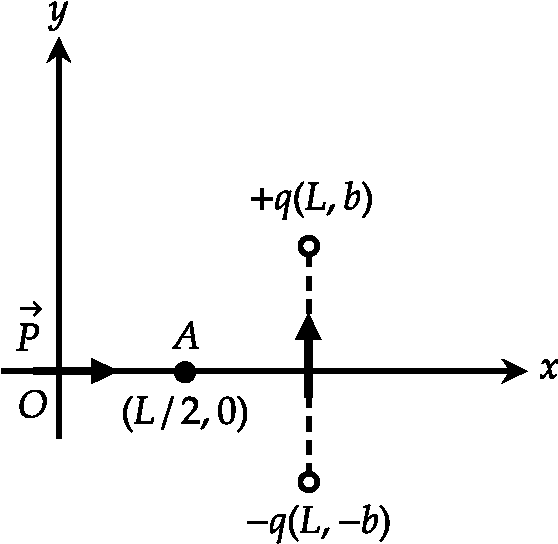
\includegraphics[height=5cm,width=5cm]{electric potential 15}
\end{figure}
\begin{tasks}(4)
	\task[\textbf{A.}] $\frac{q b}{\pi \varepsilon_{0}}\left(\frac{1}{L^{2}}+\frac{2}{L^{2}+4 b^{2}}\right)$
	\task[\textbf{B.}] $\frac{4 q b L}{\pi \varepsilon_{0}\left[L^{2}+4 b^{2}\right]^{3 / 2}}$
	\task[\textbf{C.}] $\frac{q b}{\pi \varepsilon_{0} L^{2}}$
	\task[\textbf{D.}] $\frac{3 q b}{\pi \varepsilon_{0} L^{2}}$
\end{tasks}
\end{enumerate}
 \colorlet{ocre1}{ocre!70!}
\colorlet{ocrel}{ocre!30!}
\setlength\arrayrulewidth{1pt}
\begin{table}[H]
	\centering
	\arrayrulecolor{ocre}
	\begin{tabular}{|p{1.5cm}|p{1.5cm}||p{1.5cm}|p{1.5cm}|}
		\hline
		\multicolumn{4}{|c|}{\textbf{Answer key}}\\\hline\hline
		\rowcolor{ocrel}Q.No.&Answer&Q.No.&Answer\\\hline
		1&\textbf{D} &2&\textbf{B}\\\hline 
		3&\textbf{C} &4&\textbf{C} \\\hline
		5&\textbf{A} &6&\textbf{D} \\\hline
		7&\textbf{A}&8&\textbf{B}\\\hline
		9&\textbf{B}&10&\textbf{D}\\\hline
		11&\textbf{A} &12&\textbf{B}\\\hline
		13&\textbf{D}&14&\textbf{D}\\\hline
		15&\textbf{D}&16&\textbf{C}\\\hline
		17&\textbf{C} &18&\textbf{B}\\\hline 
		19&\textbf{A} &20&\textbf{C} \\\hline
	\end{tabular}
\end{table}
\newpage
\begin{abox}
	Practise Set-2
\end{abox}
\begin{enumerate}[label=\color{ocre}\textbf{\arabic*.}]
\item An insulating sphere of radius $a$ carries a charge density
$$
\rho(\vec{r})=\rho_{0}\left(a^{2}-r^{2}\right) \cos \theta ; r<a
$$
The leading order term for the electric field at a distance $d$, far away from the charge distribution, is proportional to
{\exyear{GATE 2010}}

\begin{tasks}(4)
\task[\textbf{A.}] $d^{-1}$
\task[\textbf{B.}] $d^{-2}$
\task[\textbf{C.}] $d^{-3}$
\task[\textbf{D.}] $d^{-4}$
\end{tasks}	
\item Two charges $q$ and $2 q$ are placed along the $x$ -axis in front of a grounded, infinite conducting plane, as shown in the figure. They are located respectively at a distance of $0.5 \mathrm{~m}$ and $1.5 \mathrm{~m}$ from the plane. The force acting on the charge $q$ is
{\exyear{GATE 2011}}

\begin{figure}[H]
\centering
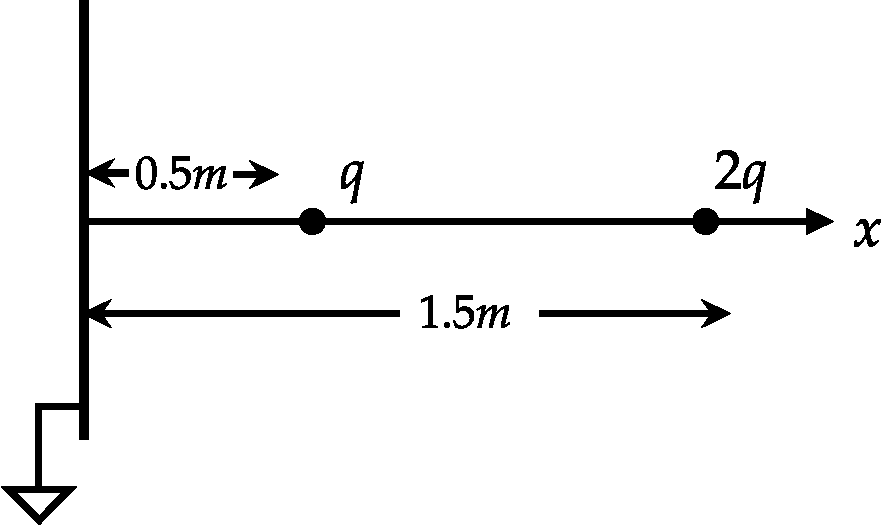
\includegraphics[height=3.5cm,width=6cm]{diagram-20210817(15)-crop}
\end{figure}
\begin{tasks}(4)
\task[\textbf{A.}] $\frac{1}{4 \pi \varepsilon_{0}} \frac{7 q^{2}}{2}$
\task[\textbf{B.}] $\frac{1}{4 \pi \varepsilon_{0}} 2 q^{2}$
\task[\textbf{C.}] $\frac{1}{4 \pi \varepsilon_{0}} q^{2}$
\task[\textbf{D.}] $\frac{1}{4 \pi \varepsilon_{0}} \frac{q^{2}}{2}$
\end{tasks}
\item A spherical conductor of radius $a$ is placed in a uniform electric field $\vec{E}=E_{0} \hat{k}$. The potential at a point $P(r, \theta)$ for $r>a$, is given by
$$
\Phi(r, \theta)=\text { constant }-E_{0} r \cos \theta+\frac{E_{0} a^{3}}{r^{2}} \cos \theta
$$
where $r$ is the distance of $P$ from the centre $\mathrm{O}$ of the sphere and $\theta$ is the angle OP makes with the $z$ -axis The charge density on the sphere at $\theta=30^{\circ}$ is
{\exyear{GATE 2011}}

\begin{figure}[H]
\centering
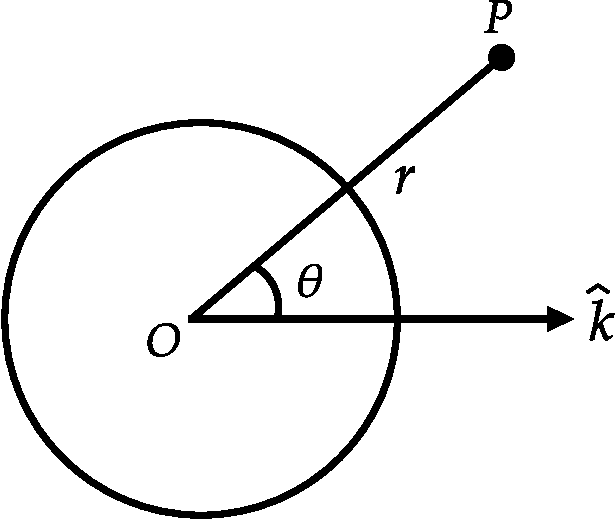
\includegraphics[height=3.5cm,width=4.3cm]{diagram-20210817(17)-crop}
\end{figure}
\begin{tasks}(4)
\task[\textbf{A.}] $3 \sqrt{3} \varepsilon_{0} E_{0} / 2$
\task[\textbf{B.}] $3 \varepsilon_{0} E_{0} / 2$
\task[\textbf{C.}] $\sqrt{3} \varepsilon_{0} E_{0} / 2$
\task[\textbf{D.}] $\varepsilon_{0} E_{0} / 2$
\end{tasks}
	\item For a scalar function $\varphi$ satisfying the Laplace equation, $\vec{\nabla} \varphi$ has
{\exyear{GATE 2013}}

\begin{tasks}(2)
\task[\textbf{A.}] Zero curl and non-zero divergence
\task[\textbf{B.}] Non-zero curl and zero divergence
\task[\textbf{C.}] Zero curl and zero divergence
\task[\textbf{D.}]  Non-zero curl and non-zero divergence
\end{tasks}
\item A charge distribution has the charge density given by $\rho=Q\left\{\delta\left(x-x_{0}\right)-\delta\left(x+x_{0}\right)\right\}$. For
this charge distribution the electric field at $\left(2 x_{0}, 0,0\right)$
{\exyear{GATE 2013}}

\begin{tasks}(4)
	\task[\textbf{A.}] $\frac{2 Q \hat{x}}{9 \pi \varepsilon_{0} x_{0}^{2}}$
	\task[\textbf{B.}] $\frac{Q \hat{x}}{4 \pi \varepsilon_{0} x_{0}^{3}}$
	\task[\textbf{C.}] $\frac{Q \hat{x}}{4 \pi \varepsilon_{0} x_{0}^{2}}$
	\task[\textbf{D.}] $\frac{Q \hat{x}}{16 \pi \varepsilon_{0} x_{0}^{2}}$
\end{tasks}
\item A charge $-q$ is distributed uniformly over a sphere, with a positive charge $q$ at its center in (i). Also in (ii), a charge $-q$ is distributed uniformly over an ellipsoid with a positive charge $q$ at its center. With respect to the origin of the coordinate system, which one of the following statements is correct?
{\exyear{GATE 2015}}

\begin{figure}[H]
	\centering
	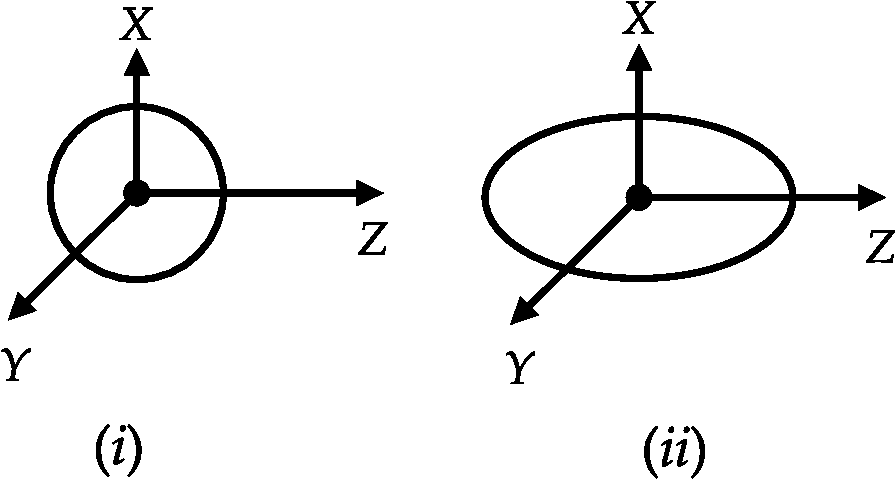
\includegraphics[height=2.5cm,width=6cm]{diagram-20210818(7)-crop}
\end{figure}
\begin{tasks}(1)
	\task[\textbf{A.}] The dipole moment is zero in both (i) and (ii)
	\task[\textbf{B.}] The dipole moment is non-zero in (i) but zero in (ii)
	\task[\textbf{C.}] The dipole moment is zero in (i) but non-zero in (ii)
	\task[\textbf{D.}] The dipole moment is non-zero in both (i) and (ii)
\end{tasks}
\item Identical charges $q$ are placed at five vertices of a regular hexagon of side $a$. The magnitude of the electric field and the electrostatic potential at the centre of the hexagon are respectively
{\exyear{GATE 2017}}

\begin{tasks}(4)
	\task[\textbf{A.}] 0,0
	\task[\textbf{B.}] $\frac{q}{4 \pi \varepsilon_{0} a^{2}}, \frac{q}{4 \pi \varepsilon_{0} a}$
	\task[\textbf{C.}] $\frac{q}{4 \pi \varepsilon_{0} a^{2}}, \frac{5 q}{4 \pi \varepsilon_{0} a}$
	\task[\textbf{D.}]  $\frac{\sqrt{5} q}{4 \pi \varepsilon_{0} a^{2}}, \frac{\sqrt{5} q}{4 \pi \varepsilon_{0} a}$
\end{tasks}
\item Three charges $(2 C,-1 C,-1 C)$ are placed at the vertices of an equilateral triangle of side $1 m$ as shown in the figure. The component of the electric dipole moment about the marked origin along the $\hat{y}$ direction is-------$C m$.
{\exyear{GATE 2017}}

\begin{figure}[H]
	\centering
	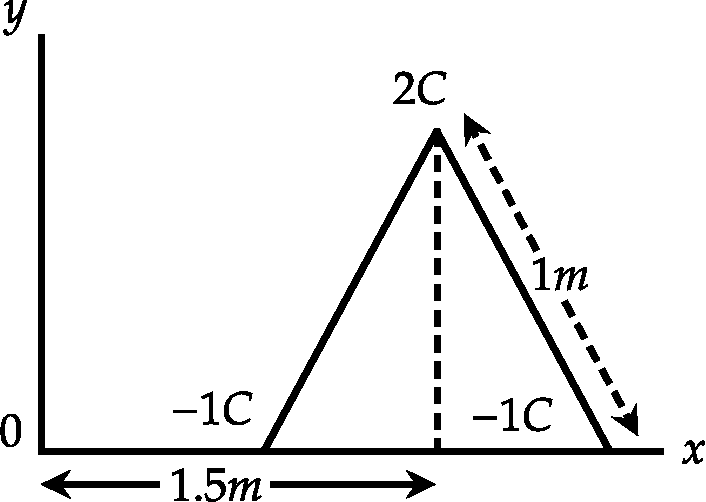
\includegraphics[height=3.5cm,width=5cm]{diagram-20210818(11)-crop}
\end{figure}
	\question Consider a system of three charges as shown in the figure below:\\
\begin{figure}[H]
	\centering
	\includegraphics[height=4.5cm,width=7cm]{diagram-20210818(17)-crop}
\end{figure}
For $r=10 \mathrm{~m} ; \theta=60$ degrees; $q=10^{-6}$ Coulomb, and $d=10^{-3} \mathrm{~m}$, the electric dipole potential in volts (rounded off to three decimal places) at a point $(r, \theta)$ is--------- [Use: $\left.\frac{1}{4 \pi \in_{0}}=9 \times 10^{9} \frac{\mathrm{Nm}^{2}}{C^{2}}\right]$
{\exyear{GATE 2019}}
\end{enumerate}
\colorlet{ocre1}{ocre!70!}
\colorlet{ocrel}{ocre!30!}
\setlength\arrayrulewidth{1pt}
\begin{table}[H]
	\centering
	\arrayrulecolor{ocre}
	\begin{tabular}{|p{1.5cm}|p{1.5cm}||p{1.5cm}|p{1.5cm}|}
		\hline
		\multicolumn{4}{|c|}{\textbf{Answer key}}\\\hline\hline
		\rowcolor{ocrel}Q.No.&Answer&Q.No.&Answer\\\hline
		1&\textbf{C} &2&\textbf{A}\\\hline 
		3&\textbf{A} &4&\textbf{C} \\\hline
		5&\textbf{A} &6&\textbf{A} \\\hline
		7&\textbf{C}&8&\textbf{1.73}\\\hline
		9&\textbf{0.045}&10&\textbf{}\\\hline
		11&\textbf{} &12&\textbf{}\\\hline
		13&\textbf{}&14&\textbf{}\\\hline
		15&\textbf{}& &\\\hline
		
	\end{tabular}
\end{table}
\newpage 
\begin{abox}
	Practise Set-3
\end{abox}
\begin{enumerate}[label=\color{ocre}\textbf{\arabic*.}]
	\item  Two charges $q$ and $-q$ are placed at $(a, 0,0)$ and $(-a, 0,0)$ respectively. Calculate electric field at $(0, a, 0)$ using electric potential.
	\begin{answer}
		Let's  find potential at a general point\ (x,y,0)\\
		
		\centering
		\includegraphics[width=0.35\textwidth]{potential pset-3-1}
		\begin{align*}
		V(x, y, 0) &=\frac{q}{4 \pi \varepsilon_{0} \sqrt{(x-a)^{2}+y^{2}}}-\frac{q}{4 \pi \varepsilon_{0} \sqrt{(x+a)^{2}+y^{2}}} \\
		V(x, y, 0) &=\frac{q}{4 \pi \varepsilon_{0}}\left[\frac{1}{\sqrt{(x-a)^{2}+y^{2}}}-\frac{1}{\sqrt{(x+a)^{2}+y^{2}}}\right] \\
		E_{x} &=-\left.\frac{\partial V}{\partial x}\right|_{x=0, y=a}
		\\&=-\frac{q}{4 \pi \varepsilon_{0}}\left[-\frac{(x-a)}{\left((x-a)^{2}+y^{2}\right)^{3 / 2}}+\frac{(x+a)}{\left[(x+a)^{2}+y^{2}\right]^{3 / 2}}\right]_{x=0, y=a}\\
		&=-\frac{q}{4 \pi \varepsilon_{0}}\left[\frac{a}{\left(2 a^{2}\right)^{3 / 2}}+\frac{a}{(2 a)^{3 / 2}}\right] \\
		&=-\frac{q}{4 \pi \varepsilon_{0} a^{2}} \cdot \frac{1}{\sqrt{2}}=\frac{q}{4 \sqrt{2} \pi \varepsilon_{0} a^{2}}\\
		E_{y} &=-\frac{\partial V}{\partial y}=-\frac{q}{4 \pi \varepsilon_{0}}\left[-\frac{y}{\left[(x-a)^{2}+y^{2}\right]^{3 / 2}}+\left.\frac{y}{\left[(x+a)^{2}+y^{2}\right]^{3 / 2}}\right|_{x=0_{0}, y=a}\right.\\
		&=-\frac{q}{4 \pi \varepsilon_{0}}\left[-\frac{a}{\left(2 a^{2}\right)^{3 / 2}}+\frac{a}{\left(2 a^{2}\right)^{3 / 2}}\right]\\
		E_{y}&=0 \\
		\vec{E}&=E_{x} \hat{i}+E_{y} \hat{j} \Rightarrow \vec{E}=-\frac{q}{4 \sqrt{2 }\pi \varepsilon_{0} a^{2}} \hat{i}
		\end{align*}
	\end{answer}
	\item An infinite number of charges each equal to $q$ are placed along the $x$ -axis at $x=1, x=4, x=8, \ldots .$ and so on.
	Find the potential at the point $x=0$ due to this set of charges.{ What will be potential if in the above set up the consecutive charge have opposite sign? }
	\begin{figure}[H]
		\begin{center}
			\includegraphics[width=0.38\textwidth]{pset2-2}
		\end{center}
	\end{figure}
	\begin{answer}
		(1) The potential at $x=0$ due to all charges is given by
		
		\begin{align*}
		V &=\frac{1}{4 \pi \varepsilon_{0} d}\left(\frac{q}{1}+\frac{q}{2}+\frac{q}{4}+\frac{q}{8}+\cdots+\infty\right) \\
		&=\frac{q}{4 \pi \varepsilon_{0} d}\left(1+\frac{1}{2}+\frac{1}{4}+\frac{1}{8}+\cdots+\infty\right) \\
		&=\frac{q}{4 \pi \varepsilon_{0} d}\left[\frac{1-\left(\frac{1}{2}\right)^{\infty}}{1-\left(\frac{1}{2}\right)}\right]=\frac{q}{4 \pi \varepsilon_{0} d}\left[\frac{1-0}{\left(1/2\right)}\right]=\frac{q}{2 \pi \varepsilon_{0} d}
		\end{align*}
		(2)When the consecutive charges are negative, then
		\begin{align*}
		V &=\frac{1}{4 \pi \varepsilon_{0} d}\left[\frac{q}{1}-\frac{q}{2}+\frac{q}{4}-\frac{q}{8}+\frac{q}{16}-\frac{q}{32}+\cdots \infty\right] \\
		&=\frac{1}{4 \pi \varepsilon_{0} d}\left[\left(\frac{q}{1}+\frac{q}{4}+\frac{q}{16}+\ldots \infty\right)=\left(\frac{q}{2}+\frac{q}{8}+\frac{q}{32}+\cdots \infty\right)\right] \\
		&=\frac{q}{4 \pi \varepsilon_{0} d}\left[\left(1+\frac{1}{4}+\frac{1}{16}+\cdots \infty\right)-\left(\frac{1}{2}+8-\frac{1}{32}+\cdots \infty\right)\right] \\
		&=\frac{q}{4 \pi \varepsilon_{0} d}\left[\left(\frac{1}{1-\left(\frac{1}{4}\right)}\right)-\frac{1}{2}\left(\frac{1}{1-\left(\frac{1}{4}\right)}\right)\right] \\
		&=\frac{q}{4 \pi \varepsilon_{0} d}\left[\frac{4}{3}-\frac{2}{3}\right]=\frac{2 q}{4 \pi \varepsilon_{0} d \times 3}=\frac{q}{6 \pi \varepsilon_{0} d}
		\end{align*}
	\end{answer}
	\item Find the potential and field along the axis of circular ring with uniform charge density $\lambda$.
	
	
	
	\opencutright
	\renewcommand\windowpagestuff{
		\centering\includegraphics[width=3.5cm]{potential pset-3-3}}
	\begin{answer}
		Let consider as elementary length on the surface.
		Therefore, the potential at the point $\mathrm{P}$ due to elementary length $d l$ is
		\begin{cutout}{1}{\dimexpr\linewidth-6cm\relax}{1pt}{1}
			\begin{align*}
			d \phi&=\frac{1}{4 \pi \varepsilon_{0}} \frac{\lambda d \ell}{\sqrt{z^{2}+a^{2}}} \\
			\phi&=\frac{\lambda}{4 \pi \varepsilon_{0}} \frac{1}{\sqrt{z^{2}+a^{2}}} \int d \ell\\
			&=\frac{\lambda}{4 \pi \varepsilon_{0}} \frac{2 \pi a}{\sqrt{z^{2}+a^{2}}}=\frac{1}{4 \pi \varepsilon_{0}} \frac{2 \pi \lambda a}{\sqrt{z^{2}+a^{2}}}\\
			&\vec{E}=-\frac{d \phi}{d z}=\frac{1}{4 \pi \varepsilon_{0}} \frac{2 \pi a \lambda z}{\left(z^{2}+a^{2}\right)^{3 / 2}} \hat{z}
			\end{align*}
		\end{cutout}
		
	\end{answer}
	\item  Find the potential a distance $r$ from an infinitely long straight wire that carries a uniform line charge $\lambda$.
	\begin{answer}
		\begin{align*}
		\text{Here, }\vec{E}&=\frac{\lambda}{2 \pi \varepsilon_{0} r} \hat{r} . \\\text{In this case we cannot set}&\text{ the reference point at $\infty$, since the charge itself extends to $\infty$. }
		\\\text{Let's set it at }r&=a\\
		\\\text{Then }V(r)&=-\int_{a}^{r}\left(\frac{1}{2 \pi \varepsilon_{0}} \frac{\lambda}{r}\right) d r=-\frac{\lambda}{2 \pi \varepsilon_{0}} \ln \left(\frac{r}{a}\right)
		\end{align*}
	\end{answer}
	\item The electrostatic potential due to a charge distribution is given by $V(r)=A \frac{e^{-\lambda r}}{r}$, where $A$ and $\lambda$ are constants. The total charge enclosed within a sphere of radius $1 / \lambda$, with its origin at $r=0$ is given by,
	\begin{tasks}(4)
		\task[\textbf{a.}]$\frac{8 \pi \varepsilon_{0} A}{e}$  
		\task[\textbf{b.}] $\frac{4 \pi \varepsilon_{0} A}{e}$
		\task[\textbf{c.}]$\frac{\pi \varepsilon_{0} A}{e}$ 
		\task[\textbf{d.}]0 
	\end{tasks}
	\begin{answer}
		
		
		\begin{align*}
		\text{We have, } V(r)&=\frac{A e^{-\lambda r}}{r}\\
		E&=-\frac{d V}{d r}=-\hat{r} \frac{d}{d r}\left[\frac{e^{-\lambda r}}{r}\right] A=\left[\frac{\lambda e^{-\lambda r}}{r}+\frac{e^{-\lambda r}}{r^{2}}\right] A \hat{r}\\
		\text{According}&\text{ to Poisson's law,}\\
		\vec{\nabla} \cdot \vec{E}&=\frac{\rho}{\varepsilon_{0}} \\
		\Rightarrow \quad \rho&=\varepsilon_{0} \vec{\nabla} \cdot \vec{E}=\varepsilon_{0} \nabla \cdot\left[\frac{\lambda e^{-\lambda r}}{r^{2}} \vec{r}+\frac{e^{-\lambda r}}{r^{3}} \vec{r}\right] A\\&=\varepsilon_{0} \lambda A \nabla \cdot\left(\frac{e^{-\lambda r}}{r^{2}} \vec{r}\right)+\varepsilon_{0} A \nabla \cdot\left(\frac{e^{-\lambda r}}{r^{3}} \vec{r}\right) \\
		&=\varepsilon_{0} \lambda A e^{-\lambda r}\left(\vec{\nabla} \cdot \frac{\vec{r}}{r^{2}}\right)+\frac{\vec{r}}{r^{2}} \varepsilon_{0} \lambda A \cdot\left(\nabla e^{-\lambda r}\right)+\varepsilon_{0} A e^{-\lambda r}\left(\vec{\nabla} \cdot \frac{\vec{r}}{r^{3}}\right)\\&+\left(A \varepsilon_{0} \frac{\vec{r}}{r^{3}} \cdot \vec{\nabla} e^{-\lambda r}\right) \\
		&=\varepsilon_{0} \lambda A e^{-\lambda r} \frac{1}{r^{2}}-A \varepsilon_{0} \lambda^{2} \frac{1}{r} e^{-\lambda r}+A \varepsilon_{0} e^{-\lambda r} 4 \pi \delta(r)-A \varepsilon_{0} \lambda \frac{1}{r^{2}} e^{-\lambda r}\\
		&=4 \pi A \varepsilon_{0}\left[\delta(r)-\frac{\lambda^{2}}{4 \pi} \frac{1}{r}\right] e^{-\lambda r} \\
		q&=4 \pi A \varepsilon_{0} \int \delta(r) e^{-\lambda r} d V-\frac{4 \pi A \varepsilon_{0} \lambda^{2}}{4 \pi} \int_{r}^{1} e^{-\lambda r} 4 \pi r^{2} d r \\
		&=4 \pi \varepsilon_{0} A-4 \pi \varepsilon_{0} A \int_{0}^{1} e^{-z} z d z \\
		&=4 \pi \varepsilon_{0} A-4 \pi \varepsilon_{0} A\left[-e^{-z} z-e^{-z}\right]_{0}^{1} \\
		&=4 \pi \varepsilon_{0} A-4 \pi \varepsilon_{0} A\left[-e^{-1}-e^{-1}+1\right]=\frac{8 \pi \varepsilon_{0} A}{e}
		\end{align*}
		
	\end{answer}
	\item The plates of a parallel plate capacitor (which are normal to the $x$ -axis) are located at $x=0$
	and $x=L .$ The plate at $x=0$ is grounded while the other plate is at a potential $V_{0} .$ The
	space between the plates has uniform volume charge density $\rho .$ The potential $V(x)$
	between the plates is given by
	\begin{tasks}(2)
		\task[\textbf{a.}]$-\frac{\rho}{2 \varepsilon_{0}} x^{2}+\left(\frac{V_{0}}{L}+\frac{\rho L}{2 \varepsilon_{0}}\right) x$  
		\task[\textbf{b.}] $\frac{\rho}{2 \varepsilon_{0}} x^{2}-\left(\frac{V_{0}}{L}+\frac{\rho L}{2 \varepsilon_{0}}\right) x$
		\task[\textbf{c.}]$-\frac{\rho}{2 \varepsilon_{0}} x^{2}-\left(\frac{V_{0}}{L}+\frac{\rho L}{2 \varepsilon_{0}}\right) x$ 
		\task[\textbf{d.}]$\frac{\rho}{2 \varepsilon_{0}} x^{2}+\left(\frac{V_{0}}{L}+\frac{\rho L}{2 \varepsilon_{0}}\right) x$
		
	\end{tasks}
	\begin{answer}
		
		\begin{align*}
		\text{ The Laplace's }&\text{equation in Cartesian coordinates system is}\\
		\nabla^{2} V&=\frac{\partial^{2} V}{\partial x^{2}}=\frac{\partial^{2} V}{\partial y^{2}}+\frac{\partial^{2} V}{\partial z^{2}}=-\frac{\rho}{\varepsilon_{0}}\\
		\text{As $V$ is only } &\text{function of $x$, we have the differential equation,}\\
		\frac{d^{2} V}{d x^{2}}&=-\frac{\rho}{\varepsilon_{0}}\\
		\text{By integrating we }&\text{have the solution of this equation as}\\
		\frac{d V}{d x}&=-\frac{\rho}{\varepsilon_{0}} x+A \Rightarrow V(x)=-\frac{\rho}{2 \varepsilon_{0}} x^{2}+A x+B \quad \text{Where $A$ and $B$ are constants.}\\
		\text{The two equations need }&\text{to be solved for the following boundary conditions:}\\
		\text{(i) }&x=0 ; V=0\\
		\text{	(ii)} &x=L ; V=V_{0}\\
		\text{Substituting these boundary }&\text{ conditions, we get,}\\
		\text { At } x&=0, V(0)=0=0+0+B \Rightarrow B=0 \\
		\text { At } x&=L, V(L)=V_{0}=-\frac{\rho}{2 \varepsilon_{0}} L^{2}+A L \Rightarrow A=\frac{V_{0}}{L}+\frac{\rho L}{2 \varepsilon_{0}}\\ \Rightarrow V(x)&=-\frac{\rho}{2 \varepsilon_{0}} x^{2}+\left(\frac{V_{0}}{L}+\frac{\rho L}{2 \varepsilon_{0}}\right) x
		\end{align*}
	\end{answer}
	\item If the electrostatic potential in spherical polar coordinates is
	$$
	\phi(r)=\phi_{0} e^{-r / r_{0}}
	$$
	where $\phi_{0}$ and $r_{0}$ are constants, then the charge density at a distance $r=r_{0}$ will be
	\begin{tasks}(4)
		\task[\textbf{a.}] $\frac{\varepsilon_{0} \phi_{0}}{e r_{0}^{2}}$  
		\task[\textbf{b.}]$\frac{e \varepsilon_{0} \phi_{0}}{2 r_{0}^{2}}$
		\task[\textbf{c.}]$-\frac{\varepsilon_{0} \phi_{0}}{e r_{0}^{2}}$ 
		\task[\textbf{d.}]$-\frac{2 e \varepsilon_{0} \phi_{0}}{r_{0}^{2}}$ 
	\end{tasks}
	
	\begin{answer}
		\begin{align*}
		\because \nabla^{2} \phi&=-\frac{\rho}{\varepsilon_{0}} \Rightarrow \rho=-\varepsilon_{0}\left(\nabla^{2} \phi\right) \\
		\nabla^{2} \phi&=\frac{1}{r^{2}} \frac{\partial}{\partial r}\left(r^{2} \frac{\partial \phi}{\partial r}\right)\\
		&=\frac{1}{r^{2}} \frac{\partial}{\partial r}\left(r^{2} \times-\frac{\phi_{0}}{r_{0}} e^{-r / r_{0}}\right)\\&=-\frac{1}{r^{2}} \frac{\phi_{0}}{r_{0}} \frac{\partial}{\partial r}\left(r^{2} \times e^{-r / r_{0}}\right) \\
		&=-\frac{1}{r^{2}} \frac{\phi_{0}}{r_{0}}\left[r^{2} \times-\frac{1}{r_{0}} e^{-r / r_{0}}+2 r e^{-r / r_{0}}\right] \\\Rightarrow \nabla^{2} \phi&=-\frac{\phi_{0}}{r_{0}}\left[-\frac{1}{r_{0}} e^{-r / r_{0}}+\frac{2}{r} e^{-r / r_{0}}\right] \\
		\text { At a distance } r&=r_{0}\\ \nabla^{2} \phi&=-\frac{\phi_{0}}{r_{0}}\left[\frac{1}{r_{0}} e^{-1}+\frac{2}{r_{0}} e^{-1}\right]=-\frac{\phi_{0}}{r_{0}^{2} e} \\\Rightarrow \rho&=-\varepsilon_{0}\left(-\frac{\phi_{0}}{r_{0}^{2} e}\right)=\frac{\phi_{0} \varepsilon_{0}}{r_{0}^{2} e}
		\end{align*}
	\end{answer}
	\item A particle of mass $40 \mathrm{mg}$ and carrying a charge $5 \times 10^{-9} \mathrm{C}$ is moving directly towards a fixed positive point charge of magnitude $10^{-8} \mathrm{C} .$ When it is at a distance of $10 \mathrm{~cm}$ from the fixed positive point charge it has a velocity of $50 \mathrm{~cm} \mathrm{sec}^{-1}$. At what distance from the fixed point charge will the particle come momentarily to rest? Is the acceleration constant during motion?
	\begin{figure}[H]
		\begin{center}
			\includegraphics[width=0.25\textwidth]{pset-3-8}
		\end{center}
	\end{figure}
	\begin{answer}
		\begin{align*}
		\text{Use conservation of energy} (K.E. + P.E.) _{\text {initial }}&=(\mathrm{K.E.}+\mathrm{P.E.})_{\text {final }}\\
		\frac{1}{2} \times 40 \times 10^{-6} \times(0.5)^{2}+\frac{10^{-8} \times 5 \times 9 \times 10^{9}}{\left(\frac{1}{10}\right)}&=0+\frac{10^{-8} \times 5 \times 10^{-9} \times 9 \times 10^{9}}{x}\\
		\text{Solving we get }r&=4.737 \times 10^{-2} \mathrm{~m}
		\end{align*}
	\end{answer}
		\item 	 A "pure" dipole $\vec{p}$ is situated at the origin, pointing in the $z$ -direction
	\\(a) What is the force on a point charge $q$ at $(a, 0,0)$ ?
	\\(b) What is the force on $q$ at $(0,0, a)$ ?
	\\(c) How much work does it take to move $q$ from $(a, 0,0)$ to $(0,0, a)$ ?
	\begin{answer}\hspace{0.5cm}
		\begin{enumerate}
			\item \begin{align*}
			A t(a, 0,0), r&=a, \theta=\frac{\pi}{2} ; \\\vec{E}&=\frac{p}{4 \pi \varepsilon_{0} r^{3}}(2 \cos \theta \hat{r}+\sin \theta \hat{\theta})=\frac{p}{4 \pi \varepsilon_{0} a^{3}} \hat{\theta} \\
			\vec{E}&=-\frac{p}{4 \pi \varepsilon_{0} a^{3}} \hat{z} \Rightarrow \vec{F}=q \vec{E}=-\frac{p q}{4 \pi \varepsilon_{0} a^{3}} \hat{z}
			\end{align*}
			\item \begin{align*}
			A t(0,0, a), r&=a, \theta=0 ;\\ \vec{E}&=\frac{p}{4 \pi \varepsilon_{0} r^{3}}(2 \cos \theta \hat{r}+\sin \theta \hat{\theta})=\frac{2 p}{4 \pi \varepsilon_{0} a^{3}} \hat{r} \\
			\vec{E}&=\frac{2 p}{4 \pi \varepsilon_{0} a^{3}} \hat{z} \Rightarrow \vec{F}=q \vec{E}=\frac{2 p q}{4 \pi \varepsilon_{0} a^{3}} \hat{z}
			\end{align*}
			\item \begin{align*}
			V_{d i p}(r, \theta)&=\frac{p \cos \theta}{4 \pi \varepsilon_{o} r^{2}} \Rightarrow V(a, 0,0)=0 \text { and } V(0,0, a)=\frac{p}{4 \pi \varepsilon_{o} a^{2}}, \\
			W&=q[V(0,0, a)-V(a, 0,0)]=\frac{p}{4 \pi \varepsilon_{o} a^{2}}
			\end{align*}
		\end{enumerate}
		
	\end{answer}
\item The electric field at a point due to an electric dipole is perpendicular to the dipole axis, the
angle between the dipole axis and the line joining the point with the centre of the dipole
is $\tan ^{-1}(\beta)$. Then the value of $\beta$ is $\ldots \ldots$.
\begin{answer}
	
	
	\begin{align*}
	\vec{E}(r, \theta)&=\frac{p}{4 \pi \varepsilon_{0} r^{3}}(2 \cos \theta \hat{r}+\sin \theta \hat{\theta}) \\
	\tan \alpha&=\frac{E_{\theta}}{E_{r}}=\frac{1}{2} \tan \theta \quad \because \alpha=90-\theta \Rightarrow \cot \theta=\frac{1}{2} \tan \theta \\
	\Rightarrow \tan ^{2} \theta&=2 \Rightarrow \theta=\tan ^{-1} \sqrt{2}
	\end{align*}
	
\end{answer}
\item Let four point charges $q,-q / 2, q$ and $-q / 2$ be placed at the vertices of a square of
side $a$. Let another point charge $-q$ be placed at the cnetre of the square (see the figure).
Let $V(r)$ be the electrostatic potential at a point $P$ at a distance $r \gg a$ from the centre of
the square. Then $V(3 r) / V(r)$ is.....................
\begin{answer} 
	\begin{align*}
	\text{The }&\text{monopole moment,}\\
	Q_{\text {mono }}&=-\frac{q}{2}+q-\frac{q}{2}+q-q=0\\
	\vec{p}&=q(a \hat{x}+a \hat{y})-\frac{q}{2}(a \hat{x}+a \hat{y})-q(a \hat{x}-a \hat{y})+q(-a \hat{x}-a \hat{y})-\frac{q}{2}(-a \hat{x}+a \hat{y})+0=0 \\
	\text { Thus } V &\propto \frac{1}{r^{3}} \Rightarrow \frac{V(3 r)}{V(r)}=\frac{1}{27}=0.037
	\end{align*}
	
\end{answer}
\item A "pure" dipole with dipole moment $\vec{p}=p_{o} \hat{z}$ is situated at the origin. A point charge $Q$ is
moved from the point $(\mathrm{a}, 0,0)$ to $(0,0, \mathrm{a})$ then the work done will be,
\begin{tasks}(4)
	\task[\textbf{a.}]  zero. 
	\task[\textbf{b.}]$\frac{p_{0} Q}{4 \pi \varepsilon_{0} a^{3}}$
	\task[\textbf{c.}] $\frac{p_{0}}{4 \pi \varepsilon_{0} a^{2}}$
	\task[\textbf{d.}] $\frac{p_{0} Q}{4 \pi \varepsilon_{0} a^{2}}$
\end{tasks}
\begin{answer}
	\begin{align*}
	W&=Q[V(0,0, a)-V(a, 0,0)]\\
	V(r, \theta)&=\frac{p_{0} \cos \theta}{4 \pi \varepsilon_{0} r^{2}}\\ \Rightarrow V(0,0, a)&=\frac{p_{0}}{4 \pi \varepsilon_{0} a^{2}} \quad \because \theta=0 \text { and } V(a, 0,0)=0 \quad \because \theta=\frac{\pi}{2}\\
	\Rightarrow W&=\frac{p_{0} Q}{4 \pi \varepsilon_{0} a^{2}}
	\end{align*}
	
\end{answer}

\end{enumerate}
